\documentclass[chapter,oneside]{oblivoir}
        
    \usepackage{graphicx}%그림을 업로드하기위한 패키지

    %\usepackage{ikps} %일격필살에서 배포한 패키지
    \usepackage{tabu}

    \usepackage{multirow} 

    \usepackage{enumitem}
    %\usepackage[table,dvipsnames]{xcolor}  %table 색을 쓰기위한 패키지
    \usepackage{dhucs-enumitem} %kotex enumerate 가. 를 쓰기위한 패키지

    \usepackage{syntonly}
    %\syntaxonly
    %\usepackage{urlbst}
    %%%%%%%% for itemize in tabu :  https://tex.stackexchange.com/questions/381625/lists-in-tabu-environment
    \usepackage{etoolbox}
    \usepackage{url}
    \AtBeginEnvironment{tabu}{\setlist[itemize]{wide = 0pt, leftmargin = *}}

%참고문헌 관련 : http://cfs5.tistory.com/upload_control/download.blog?fhandle=YmxvZzQ5OTI4QGZzNS50aXN0b3J5LmNvbTovYXR0YWNoLzAvMTIwMDAwMDAwMDAwLnBkZg%3D%3D
% http://wiki.ktug.org/wiki/wiki.php/%EC%B0%B8%EA%B3%A0%EB%AC%B8%ED%97%8C
% http://www.ptep-online.com/ctan/lshort_korean.pdf
    
\makeatletter
    \newcommand*{\compress}{\@minipagetrue}
    \newcommand{\spec}{
    \begin{itemize}
        \item OS : windows 10 / 64bit
        \item CPU : gtx 1060 6GB
        \item GPU : i7 - 7700
        \item RAM : 16GB
    \end{itemize}
    }
    \makeatother
%더해야할것 그래픽스,타부, 타이틀 

\begin{document}
\begin{center}
	
	{\scshape\LARGE 최 종 연 구 보 고 서 \par}
	\vfill
	{\scshape\Large 연구 제목 \par}
%	\vspace{1.5cm}
\vfill
\vfill
	{ 부경대학교\par}
	
	%{\Large\itshape John Birdwatch\par}
    \vfill
    
	한 국 전 자 통 신 연 구 원

	\vfill

% Bottom of the page
%    {\large \today\par}
    
\end{center}

\newpage
\begin{center}
    최 종 연 구 보 고 서
    \vfill
    연구 제목
    \vfill
    부경대학교
    \vfill
    한 국 전 자 통 신 연 구 원
    \vfill
    제     출     문
    \vfill    
    
    한국전자통신연구원장  귀하
    \vfill
    본 보고서를 연구제목의 최종연구보고서로 제출합니다. 
    
\vfill
2018년 12월 일\par
\end{center}

\vfill
\vspace{0.5cm}
수  탁  기  관 :  부경대학교 산학협력단\par
\vspace{0.5cm}
수 탁 기 관 장 :           (인)\par
\vspace{0.5cm}
연 구 책 임 자 :  \par
\vspace{0.5cm}
참 여 연 구 원 :  \par

\newpage


\begin{center}
    {\scshape\LARGE 요약문 \par}    
\end{center}


{\Large\textbf{1. 제   목 : 연구 제목}  \par}
\vspace{1cm}
{ \Large\textbf{2. 연구의 목적 및 중요성} \par}
\vspace{1cm}
\textbf{연구의 목적}

얼굴인식 및 얼굴합성 기술을 구현하고 COX 서버에서 네 가지 기술들(Zad,Deepfake,Openpose,GAN)을 동작하게 하고 사용자가 원하는 사진과 영상을 가지고 서버에서 Faceswap이 가능하게 하는 것이다. 

두 번째 목적은 COX Cinema 영상제작자가 만든 영상을 단지 사용자에게 보여주는 단방향적인 방식이 아닌 영상제작자가 사용자에게 여러 선택권을 주고, 사용자로 하여금 영상의 진행을 선택하여 영상을 시청하게 하는 것이 가능하게 하는 것이다. 

\textbf{전체 연구목표}

\begin{itemize}
    \item 얼굴인식 및 얼굴합성 기술의 구현과 COX 서버에서의 기술 작동

세부목표1 : 네 가지 기술(Zad,Openpose,Deepfake,GAN) 구현

\item 2D-Faceswap(Zad) 모델 기술 구현

\item Openpose 기술 구현

\item Deepfake(Original-High-Resolution Model) 기술 구현 

\item 생성적 적대 신경망(GAN) 기술 구현 

세부목표 2 : 서버 구축 및 네 가지 Faceswap 기술이 서버에서도 작동되게 하는 것이다.

\item COX서버 구축 (우분투?)

\item 네 가지 기술 IN COX Page

세부목표 3 : COX Cinema 

\item 사용자의 휴대폰 기기와 웹에서의 영상 사이에 Interactive 기능 삽입
    
\end{itemize}

\textbf{연구의 중요성}

최근 Face Swap 기술의 관심이 높아지고 있으며 특히 SNOW(NAVER)나 Meitu(중화인민공화국)에서 얼굴 인증 시스템을 이용하여 가공 및 합성하는 뷰티 카메라가 큰 인기를 끌고 있다. Face Swap 기술을 상용화한 COX는 유튜브나 트위치 같은 거대 플랫폼처럼 만들 수 있는 기회가 될 수 있는 교보재가 될 수 있다.

\vspace{1cm}

{ \Large\textbf{3. 연구의 내용 및 범위}  \par}
\vspace{0.5cm}

{ \large\textbf{3.1 연구 내용}  \par}

\vspace{0.5cm}

Deep Learning을 이용한 얼굴인식 및 얼굴 합성 기술

\vspace{0.5cm}

{\large\textbf{3.2 연구에 쓰인 범위}  \par}

\begin{itemize}
   \item  Python (version 3.6) 
   \item PHP (version 5.6) 
   \item C++    
\end{itemize}


{\Large\textbf{ 4. 연  구  결  과}  \par}

\vspace{0.5cm}

COX 페이지에서 네 가지 기술
\begin{itemize}
    \item Zad
    \item Openpose
    \item Deepfake
    \item GAN
\end{itemize}
을 구현 가능하게 하였다. 서버에서 돌아가게 만들었으며 실시간으로 사용이 가능하다. 기존의 COX를 구현할 때에는 많은 영상이 있어야 하는데 그러한 단점들을 보완하여, 기존의 영상들을 재사용하고 최신기술을 접목하여 창의적인 영상을 만들 수 있게 하였다.

\vspace{1cm}

{\Large\textbf{ 5. 활용에 대한 건의}  \par}
\vspace{0.5cm}

본 연구결과는 COX페이지에서 Face Swap이라는 주제로 한 챕터를 차지할 수 있다. 이용자들은 Face Swap을 이용하여 자신이 원하는 영상과 사진으로 Face Swap을 이용할 수 있다.

두 번째로 COX Cinema 플랫폼은 이용자가 COX Cinema의 인터랙티브 기능을 이용하여 여러 재미있는 영상을 만들 수 있다. 

세 번째로는 COX Cinema 플랫폼을 이용하여 교육영상이나 광고에 활용될 수 있다.


\vspace{1cm}
{\Large\textbf{ 6. 기  대  효  과} \par}

\vspace{0.5cm}

본 연구결과는 네 가지 기술의 서버 시스템 상에서의 구현을 통해 여러 가지 기대효과를 얻을 수 있다고 생각하였다. 첫 번째로 기술적 기대효과이다. Rendering 기술과 Deep Learning 기술을 통하여 얼굴 인증 및 합성을 통해 영상을 재사용하는 핵심 기술로 활용되는 것이다.
두 번째로 기술이전을 통한 기대효과이다. 얼굴인식 / 인증 분야 활용을 통한 다른 외산 제품으로의 수입대체사용 (ex. SNOW, Meitu) Faceswap 기술을 요소 기술로 활용하여 더 나은 이미지와 영상으로의 부가가치 제고를 가능하게 할 수 있다.

세 번째로 경제적 기대 효과이다. 얼굴인식, 얼굴교환기술 분야에서의 활용을 통한 내수 시장을 공략할 수 있을 것으로 기대된다. 뿐만 아니라 결과물 상용화 시점에서 연간 100억(
모름) 이상의 수출 효과를 낼 수 있을 것으로 보인다.

\newpage
%\include{summary.tex}
%\includegraphicx{summary.pdf}
%\includegraphics{summary.pdf}
\include{summary.pdf}


% -   목     차   -

% 제  1  장 얼굴모양 추출, 얼굴 추적, 얼굴영역 변형 기술 동향 분석

% 제  1  절 얼굴교체 기술의 요소기술

% 제  2  절 얼굴교체 기술 국내외 연구동향

% 제  2  장 2D-Faceswap 모델의 기술 분석 및 구현

% 제  1  절 2D-Faceswap 모델의 개요와 얼굴 합성 알고리즘 분석

% 제  2  절 2D-Faceswap 모델의 분석

% 제  3  절 2D-Faceswap 모델의 테스트 환경 및 결과

% 제  3  장 Openpose를 활용한 Faceswap 모델의 기술 분석 및 구현

% 제  1  절 Openpose 얼굴 변형 모델의 개요와 얼굴 합성 알고리즘 분석

% 제  2  절 Openpose 얼굴 변형 모델의 테스트 환경 및 결과

% 제  4  장 딥페이크(Original-High-Resolution Model)의 기술 분석 및 구현

% 제  1  절 딥페이크의 개요와 얼굴 합성 알고리즘 분석

% 제  2  절 딥페이크 내의 모델 분석

% 제  3  절 딥페이크 모델의 테스트 환경 및 결과

% 제  5  장 생성적 적대 신경망(GAN)을 활용한 Faceswap 모델의 기술 분석 및 구현

% 제  1  절 GAN을 활용한 얼굴 변형 모델의 개요와 얼굴 합성 알고리즘 분석

% 제  2  절 GAN을 활용한 얼굴 변형 모델 분석

% 제  3  절 GAN을 활용한 얼굴 변형 모델의 테스트 환경 및 결과

% 제  6  장 서버(Server)를 통한 위 네 가지 기술의  연결 과정?구현? 및 결과  

% 제  1  절 구현한 서버 

% 제  2  절 2D-Faceswap 모델 코드 분석

% 제  3  절 Openpose 를 활용한 Faceswap 모델 코드 분석

% 제  4  절 딥페이크(Original-High-Resolution Model) 코드 분석

% 제  5  절 생성적 적대 신경망(GAN) 코드 분석

% 제  7  장 COX 서버 구축 및 OOO(형식) 광고 동영상 제작 및 업로드

% 제  1  절 COX 서버 설명

% 제  2  절 

% 제  3  절 

\tableofcontents
\newpage

\listoftables
\newpage

\chapter{얼굴모양 추출, 얼굴 추적, 얼굴영역 변형 기술 동향 분석 }

\section{얼굴교체 기술의 요소기술}

\subsection{ 얼굴교체(Face Swapping) 기술의 정의}

얼굴 교체(Face Swapping)기술이란 원본(source) 사진의 얼굴을 대상(target) 사진에 나타나는 얼굴로 옮겨 현실적이고 편집되지 않은 결과를 얻으려고 시도하는 것을 의미한다. 최근에는 Deep Learning 기술의 발전에 따라서 이에 기반한 연구가 활발히 진행되고 있다.

\subsection{ 얼굴교체(Face Swapping)기술의 사용용도}

얼굴 교체 기술은 다음과 같은 용도로 사용될 수 있다.

\begin{itemize}
    \item 자신이 좋아하는 사진이나 동영상에 본인의 얼굴을 입혀 자신만의 콘텐츠를 제작할 수 있다.
    \item 영화 또는 드라마에 자신이 좋아하는 연예인의 얼굴을 입혀 본인만의 영화와 드라마를 감상할 수 있다.
    \item 보안 유지, 얼굴 데이터 변형(face specific data augmentation method) 에도 사용될 수 있다.
\end{itemize}

\subsection{ 얼굴교체(Face Swapping)기술의 요소 기술}

얼굴 교체 기술은 세부적인 기술 요소에 상관없이 그림 1에 보인 대략적인 순서도의 절차를 따르게 된다. 최근 활발한 연구가 이루어지고 있는 Deep Learning기반의 얼굴 교체 기술 또한 마찬가지이다. 

\begin{figure}[h!]
  \centering
    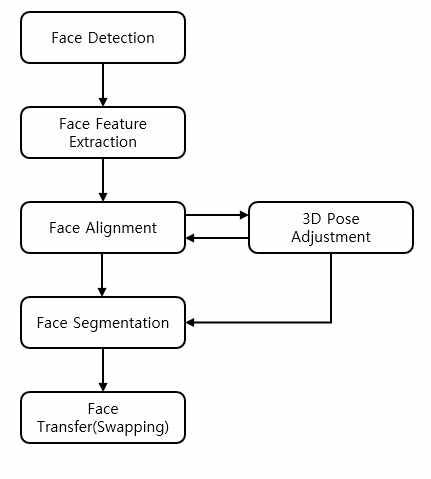
\includegraphics{pic/chp1/img371}
  \caption{얼굴 교체 순서도}
\end{figure}

다음은 대략적으로 얼굴 교체에 사용되어 지고 있는 요소기술을 설명한다.

                        
\begin{enumerate}%[label={\pgana*.}]
    \item  얼굴 검출(Face Detection)

    얼굴 검출 요소 기술은 사진 또는 동영상 내에 존재하는 얼굴의 위치를 bounding box를 이용하여 검출하게 된다. 이를 이용하여 검출된 얼굴위치(영역)은 이후 사후처리에 도움을 주게 된다.

    \begin{figure}[h!]
        \centering
        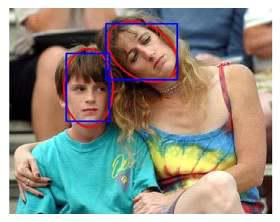
\includegraphics{pic/chp1/img398}
        \caption{얼굴영역 검출\cite{reference1}}
    \end{figure}
            
    \item 얼굴 특징점 추출 (Face Feature Extraction)

    얼굴 특징점 추출 요소 기술은 얼굴영역의 주요 지점(눈, 코, 입, 눈썹, 턱선, 귀 등)을 추출하는 기술을 의미한다. 얼굴을 표현(face representation)하는데에 있어서 기준이 되는 점들이다.
    \begin{figure}[h!]
        \centering
        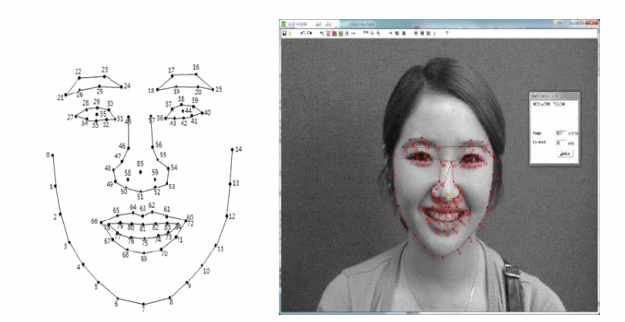
\includegraphics{pic/chp1/img399}
        \caption{얼굴 특징점 추출\cite{reference2}}
    \end{figure}

    \item 얼굴 정렬 기술 (Face Alignment)

    얼굴 정렬 요소 기술은 이미지를 통해 얼굴 표식의 위치를 얻는 과정이다. 이는 향후 얼굴 인식(face recognition)과 같은 사후에 적용될 기술에 영향을 끼치게 된다.
    \begin{figure}[h!]
        \centering
        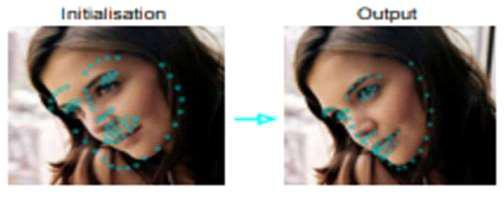
\includegraphics{pic/chp1/img400}
        \caption{얼굴 정렬 기술\cite{reference3}}
    \end{figure}

    \item 얼굴 영역 분할 기술(Face Segmentation)

    얼굴 영역 분할 요소 기술은 얼굴을 교체하기 위해 얼굴이 아닌 나머지 영역을 제외하는 기술이다.

    \begin{figure}[h!]
        \centering
        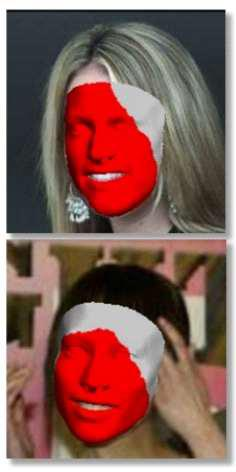
\includegraphics{pic/chp1/img427}
        \caption{ 얼굴 정렬 기술\cite{reference3}}
    \end{figure}

    \begin{figure}[h!]
        \centering
        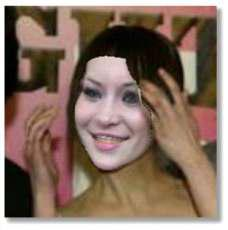
\includegraphics{pic/chp1/img428}
        \caption{얼굴 정렬 기술\cite{reference3}}
    \end{figure}

    그림5  얼굴 분할 기술\cite{reference4}

    \item 얼굴 전이기술(Face Transfer)

    얼굴 전이 요소기술은 하나의 얼굴을 본따서 다른 얼굴에 그대로 전이시키는 기술이다. 원본 얼굴의 특색을 살리면서 전이가 가능하지만, 약간의 부자연스러움을 느낄 수 있다.
    \begin{figure}[h!]
        \centering
        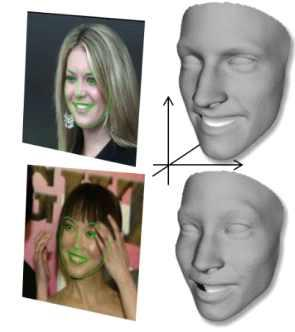
\includegraphics{pic/chp1/img435}
        \caption{얼굴 전이 기술\cite{reference4}}
    \end{figure}

    \item  3차원 자세조정기술(3D Pose Adjustment)

    3차원 자세조정 요소기술은 3차원 모델을 매개체로 하여 얼굴을 정렬하게 된다. 2D에 비해 더욱 견고(robust)한 모델이며, 훨씬 자연스러운 결과를 얻을 수 있다. 

    \begin{figure}[h!]
        \centering
        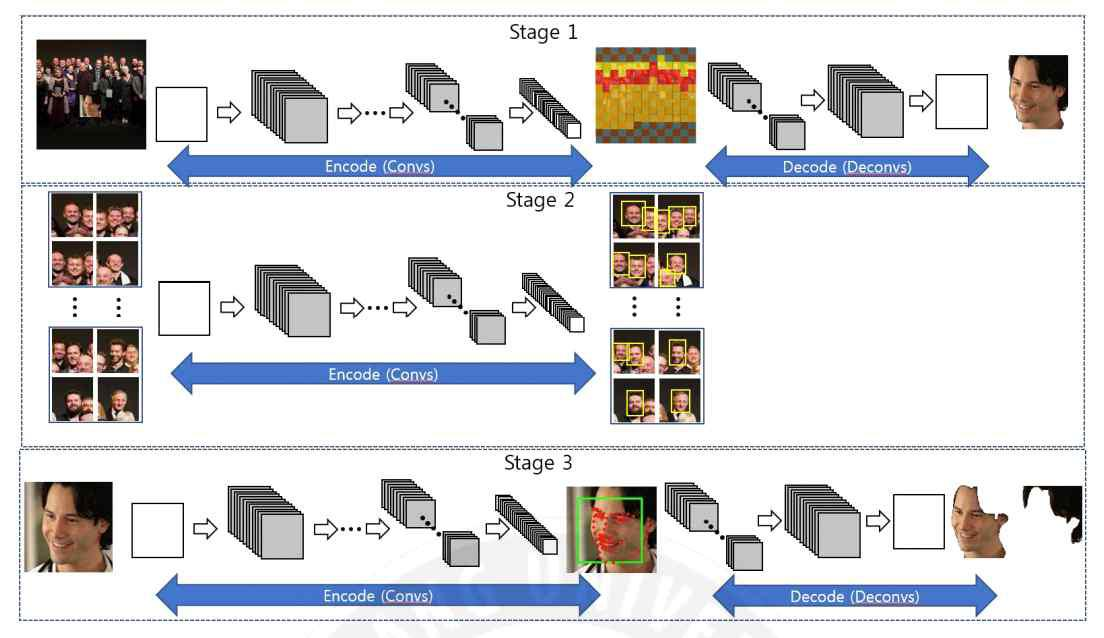
\includegraphics{pic/chp1/img496}
        \caption{ 3차원 자세 조정\cite{reference4}}
    \end{figure}
\end{enumerate}

\section{얼굴교체 기술 국내외 연구동향}

\subsection{얼굴 검출 및 특징점 추출 기술 관련 최근 국내외 연구동향}

얼굴 검출 및 특징점 추출 기술 관련 국내외 연구동향은 Deep Learning에 기반한 연구가 상당히 증가하였다. 다음 사진은 각 시기별 기술과 정확도(LFW)를 나타낸다. 또한 Deep Learning에 기반한 연구는 3년만에 99.8\%의 정확도를 달성하였다.[6]


\begin{figure}[h!]
\centering
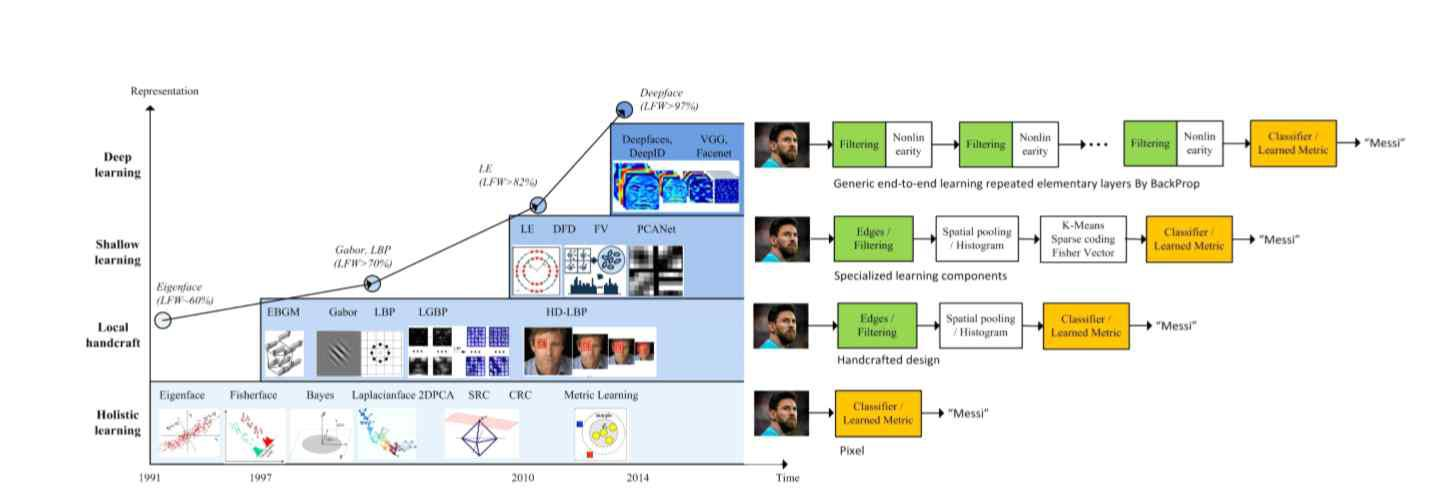
\includegraphics[scale = 0.7]{pic/chp1/img497}
\caption{ 시기 별 기술과 정확도(LFW) \cite{reference6}}
\end{figure}


\begin{enumerate}%[label={\pgana*.}]
    \item 한양대학교 :

    Deep Learning 모델인 SGNet을 사용하여 실시간으로 얼굴 및 랜드마크 검출을 위한 DCNN을 최적화하는 설계를 개발하였다. 
    상호보완이 가능한 얼굴 검출 DCNN 2가지를 모으고, Sliding window 방식이 아닌 Grid 방식을 이용하여 효율을 높였다. 
    또한, 큰 얼굴을 전문적으로 찾아내는 DCNN, 작은 얼굴을 전문적으로 찾아내는 DCNN, 마지막으로 각 얼굴의 랜드마크를 찾아내는 DCNN과
    같이 깊은 DCNN을 설계하는 대신 3단계 네트워크로 나누어서 설계하였다. 비교 대상으로, 
    얼굴 검출 알고리즘 중에서 효율적인 알고리즘이라고 알려져 있는 MTCNN과 비교했을 때, 66배의 속도 향상과 약 20\%의 검출률 향상률이 있었다.

    \begin{figure}[h!]
        \centering
        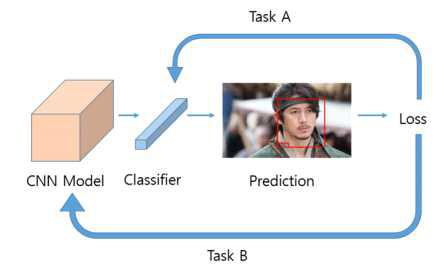
\includegraphics[scale = 0.7]{pic/chp1/img522}
    \end{figure}

    \item 서강대학교 : 

    얼굴 교체 연구에서 아시아인 교체에 대한 결과가 좋지 않은 연구가 서양인에 비해 상대적으로 많다.
    이에 관련하여 연구진들은 한국 연예인 얼굴 데이터셋을 모아 실험을 하였고, 
    FaceNet의 Fine-Tuning을 통해 연예인 1000명을 대상으로 얼굴 검출을 한 뒤, 
    91.3\%의 정답률을 보이는 결과를 얻었다.

    \begin{figure}[h!]
        \centering
        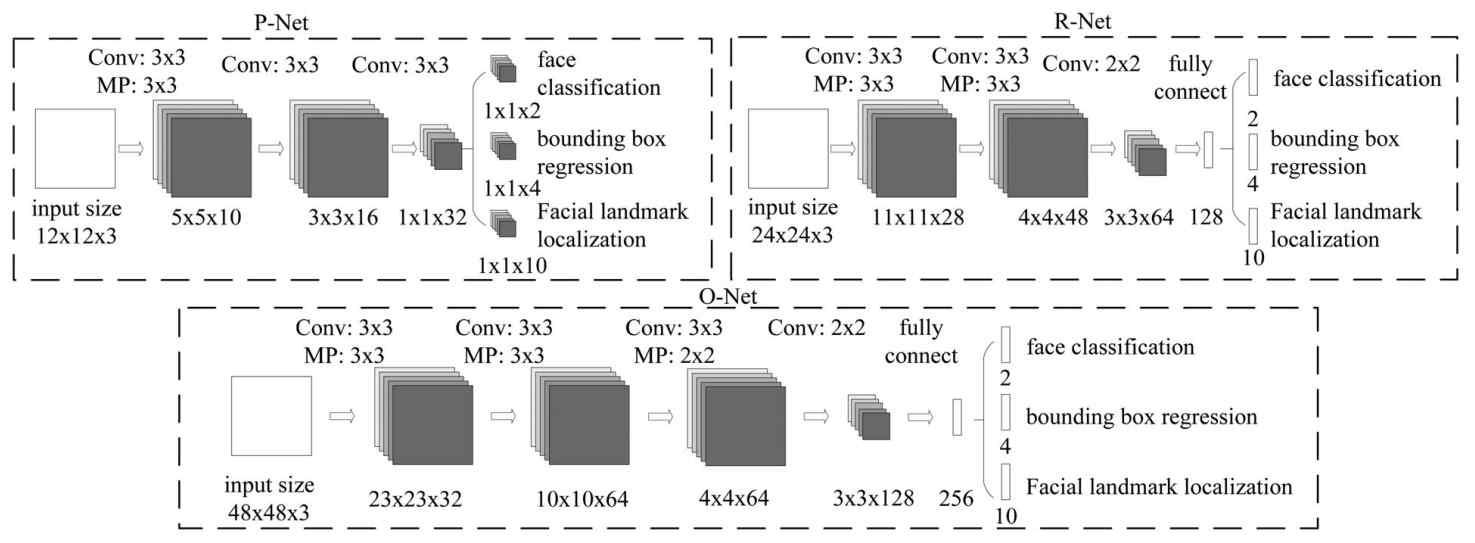
\includegraphics[scale = 0.7]{pic/chp1/img523}
    \end{figure}

    \item Joint Face Detection and Alignment Using Multitask Cascaded Convolutional Networks : 

    제약되지 않은 환경(다양한 포즈, 그림자, 배경)에서의 얼굴 검출과 정렬은 매우 어려운 작업이다. 
    이들은 Computer Vision에서 가장 많이 사용되는 CNN을 활용하여 이를 극복하는 것을 시도하였다.
    Bounding box regression을 사용하여 얼굴의 특징을 파악하게 되는데, 이때 P-Net, R-Net, O-Net이 사용된다.
    ‘MTCNN’이라고 불리우며 현재까지 가장 효율적인 얼굴 검출 알고리즘이라고 알려져 있으며, 여러 연구에서 많이 사용하고 있다. 

    \begin{figure}[h!]
        \centering
        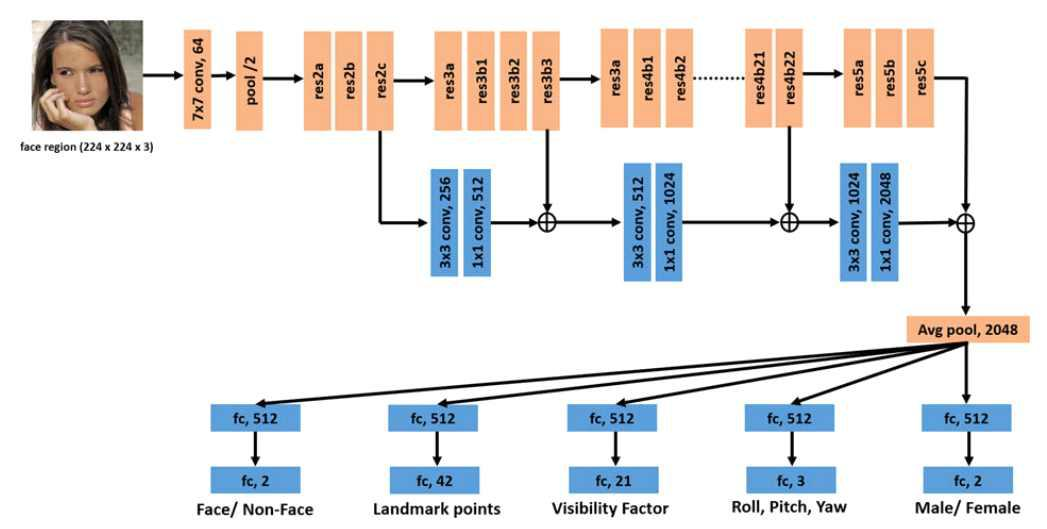
\includegraphics[scale = 0.7]{pic/chp1/img530}
    \end{figure}

    \item HyperFace: A Deep Multi-Task Learning Framework for Face Detection, Landmark Localization, Pose Estimation, and Gender Recognition : 

    이 연구는 CNN을 사용하여 얼굴 검출, 얼굴 특징점의 지역화, 행위 추정, 성별 인지를 동시에 하는 알고리즘을 개발하였다. 
    Deep Learning의 성능을 최적화 시키기 위한 가장 효율적인 네트워크인 ResNet-101을 기반으로 하였고, R-CNN의 기법인 region proposals를 사용하여 속도를 높였다. 
    정확도, 속도 측면에서 (다) 방법에 비해 2배가량 향상된 결과를 보여주었다. 

    \begin{figure}[h!]
        \centering
        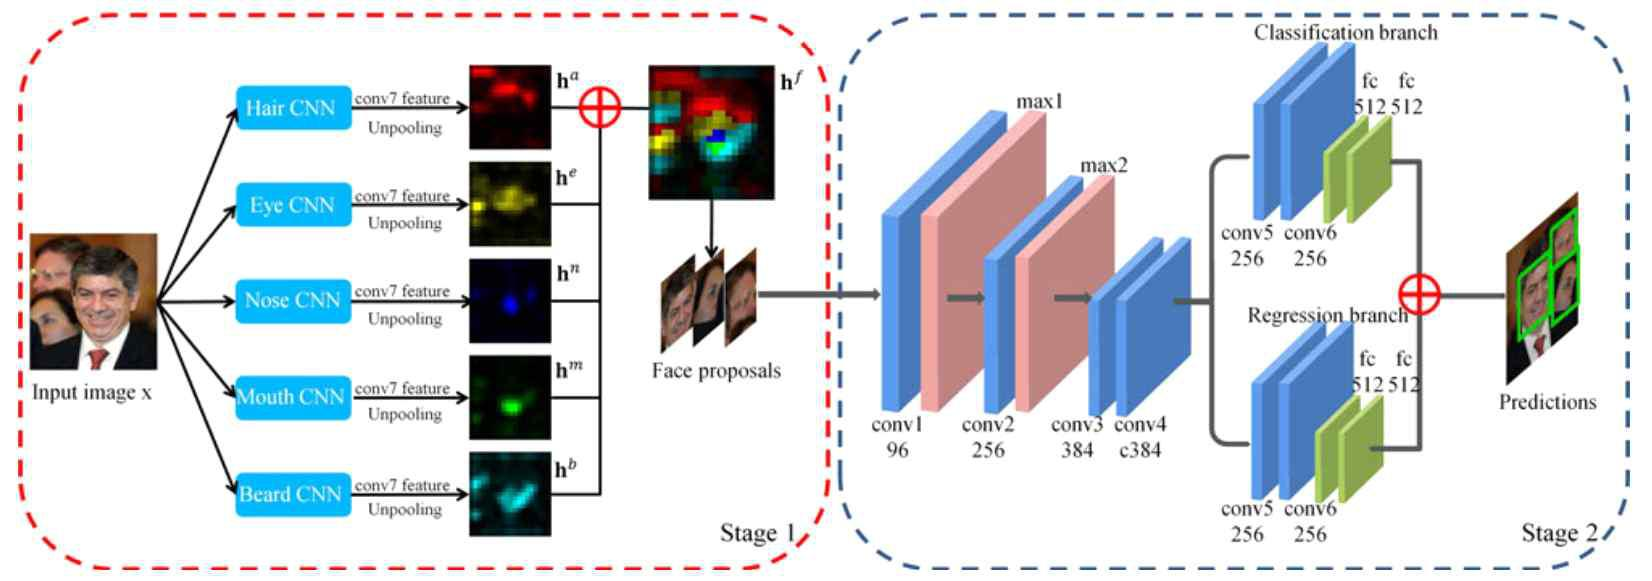
\includegraphics[scale = 0.7]{pic/chp1/img552}
    \end{figure}

    \item Faceness-Net: Face Detection through Deep Facial Part Responses : 

    이 연구는 얼굴의 특정 부위 별로 학습된 CNN을 활용하여 정렬되지 않은 얼굴 사진에서의 얼굴 검출을 성공적으로 해낸 연구이다. 
    관련 그림과 같이 총 2가지 stage로 나뉘어져 있다. 첫번째 단계는 각각 다른 얼굴 부위(머리, 눈, 코, 입, 턱)에서의 반응 맵을 생성가능한 CNN으로 이루어져있다. 
    각각의 반응 맵은 특정 부위의 영역에 맞게 활성화되어 있음을 볼 수 있다. 
    두번째 단계는 MTCNN을 통해 얼굴 분류, Bounding box regression을 최적화하여 최종적으로 얼굴의 위치를 검출합니다. 

\end{enumerate}

\subsection{ 얼굴 검출 및 특징점 추출 기술의 분류 및 특징 }

최근에 Deep Learning 기반의 end-to-end 알고리즘에 대한 연구가 활발해지면서 대표적으로 2가지 분야로 나뉘어지게 되었다. 1) Filter-based 2) Deep Learning-based

\subsubsection{Filter-based}

최근 Filtering 알고리즘에서는 대부분 LBP(Local Binary Pattern)으로 대체되어졌다. 하지만 이미지 그대로에 LBP를 적용할 경우 노이즈(noise)와 큰 변형(large variation)으로 인해 원하는 결과를 얻기 힘들 것이다. 따라서 Filtering 분야에서는 2가지 Phase로 나누어서 진행하게 된다. Phase1에서는 Filter에 관련된 알고리즘(대부분 histogram을 얻는 HOG 방식을 따른다)을 사용한 뒤, 후처리를 진행한다. 이와 관련된 알고리즘으로서는 대표적으로 Gabor Filter가 있으며, 이를 변형한 Log-Gabor, Gabor magnitude, Gabor Volume 등도 사용되며 Local edge through different orientations, Discriminantly filtered image도 사용된다. Phase2에서는 이렇게 전처리 된 이미지를 LBP를 사용하여 얼굴 특징을 추출하게 된다.
\iffalse
\begin{table}[h!]
\centering
\begin{tabular}{|c|c|}
    \hline
    \rowcolor{lightgray} Phase 1 & Phase 2 \\ \hline
    Gabor magnitude & LBP \\ \hline
    Gabor magnitude + phase  & LBP \\ \hline
    Log-Gabor &  LBP \\ \hline
    Gabor magnutude  & LBP \\ \hline
    Local edge through different orientations &  LBP \\ \hline
    Sobel or Gabor + Sobel & LBP \\ \hline 
    Gabor Volume  & LBP \\ \hline
    Discriminantly filtered image & LBP \\ \hline
    \hline
\end{tabular}
\caption{Openpose의 인터프리터 셋팅 }
\end{table}
\fi
\subsubsection{ Deep Learning-based}

앞서 설명한 Filter-based 방식에서의 단점은 제약이 있는 상황(constraint circumstance)에서만 좋은 결과를 얻는다는 것이다. 예를 들어, illuminate, pose 등의 복합적인(제약이 없는 – unconstraint circumstance) 상황이 추가되면 얼굴 특징을 잘 추출하지 못한다. 이러한 점을 해결하기 위해 연구자들은 주로 Deep Learning 알고리즘(대표적으로 CNN)을 사용하고 있다. 또한 얼굴 검출(인식) 및 특징점 추출 관련 기술에서는 이미 Deep Learning에 기반한 기술이 이전 기술(ex: Filter-based)에 비해 99\%의 정확도를 보이는 등 상당히 좋은 결과를 보이고 있어 이제는 관련 기술 연구에 있어서는 Deep Learning을 필수적으로 사용하게 되었다.
\begin{center}
\begin{tabu} to \linewidth{|X[1,c,m]|>{\compress}X[3.5,c,m]|}%
    \tabucline-%
    %%%%% 1st row
    Framework & Details \\ \tabucline-
    %%%%% 2nd row
    %%%%% 2-1 
CNN 
    &%
    %%%%% 2-2
    \begin{itemize}
        \item output layer directly connected with the penultimate and antepenultimate layer 
        \item bilinear CNN 
        \item 5-layer CNN + multitasking  
        \item frontal alignment by 3D face +  7 layer CNN 
        \item CNN with feature sharing  
        \item joint feature projection learning  
        \item supervisory signals involved  
        \item two lightened CNN models with MFM, inception layer and stacked convolution 
        \item one CNN for canonical view recovery and another CNN for feature extraction  
        \item CNNs combined with stacked auto-encoder 
    \end{itemize}
    \\ \tabucline-
    \end{tabu}
\end{center}

\section{얼굴 교체 및 인식 기술 관련 최근 국내외 연구동향}

얼굴 교체 기술 관련 최근 국내외 연구동향 또한, Deep Learning에 기반한 연구(특히 GAN : Image-to-Image translation)가 증가하였다. 이에 관련한 기관 연구(사업)에 대한 내용과 관련 연구를 설명한다.


위 사진은 연도별로 좋은 성능을 보인 논문을 정리해 놓은 것이다. 2015년 이후로 모델에 관련된 연구보다는 Loss 관련 연구로 분위기가 넘어간 것이 보이는데, 이를 citation에 근거하여 설명할 수 있다. 각 연도별 state-of-art 논문의 citation수를 $>1500$, $> 500$. $> 100$ 단위로 나누어서 구분해 보았다. 

\begin{figure}[h!]
  \centering
    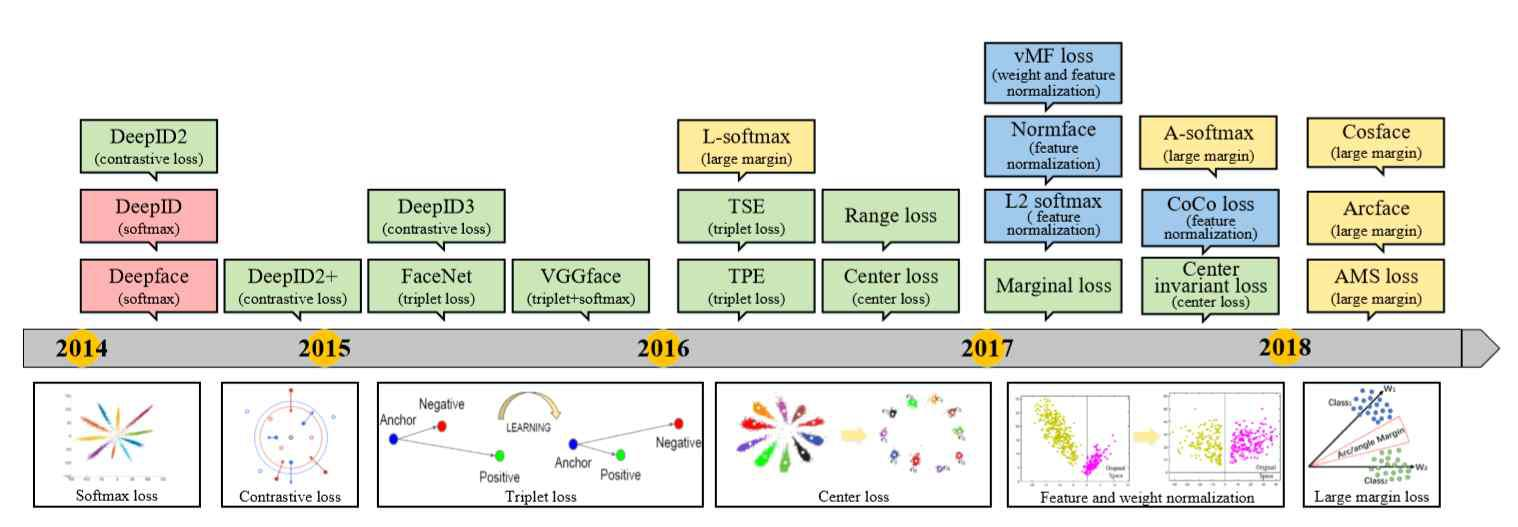
\includegraphics[scale = 0.7]{pic/chp1/img594}
  \caption{연도 별 연구 동향 \cite{reference6}}
\end{figure}

\begin{itemize}
\item   citation $> 1500$ : Deepface, FaceNet, VGGFace
\item   citation $> 500$  : DeepID2, DeepID, Center loss
\item   citation $> 100$  : DeepID2+, DeepID3, L-softmax, A-softmax
\end{itemize}

주로 1500이 넘는 인용수를 가지는 논문은 15~16년도에 집중되어 있는 것을 볼 수 있는데, 이 현상이 최근 얼굴 관련 연구 동향이 바뀌었다는 것을 설명하여 준다. 실제로 최근 연구되어지고 있는 GAN에서 대부분 얼굴 검출 또는 특징점 추출 과정에서 VGGFace나 FaceNet을 주로 사용하는 것을 볼 수 있다. 

다음은 그 외의 내용을 설명한다.
\begin{enumerate}%[label={\pgana*.}]

\item NAVER : 네이버는 최근 이미지, 음성인식, 자연어 처리 등에서 우수한 성적을 거두고 있으며, 특히 자연어 처리 분야에서 세계 1위의 자리를 차지할 만큼 AI에 대한 투자가 활발하다. 이에 얼굴 관련해서는 웹툰을 이용하여 소비자들에게 실험적으로 선보인 만화가 있다. 네이버 웹툰 ‘마주쳤다’ 는 독자의 사진을 활용해 웹툰 이미지로 생성했으며 독자가 웹툰 속 주인공이 되는 경험을 제공했다. 또한, 네이버 ‘D2 스타트업 팩토리’에 입주한 스타트업 알레시오는 GAN을 응용해 태아의 입체 초음파 사진을 생후 아기의 얼굴로 변환해주는 서비스를 준비 중이다.

\begin{figure}[h!]
    \centering
      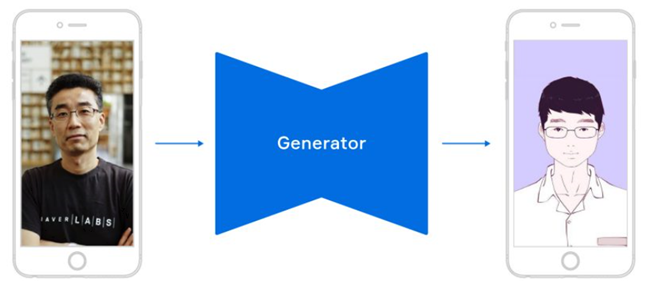
\includegraphics[scale = 0.5]{pic/chp1/imgnaver}
    \caption{ GAN을 활용한 네이버 웹툰 ‘마주쳤다’ \protect\footnote{출처: 네이버랩스}}
\end{figure}


\item 미국 워싱턴 대학교 : 워싱턴 대학교의 연구진은 버락 오바마 전 미국 대통령의 가짜 영상을 만들어냈다. 오바마 전 대통령의 연설 영상에서 음성을 따서 이 음성에 맞게 입모양을 내도록 학습시켜 합성해 실제로는 존재하지 않는 영상을 만들어냈다. 

\begin{figure}[h!]
    \centering
      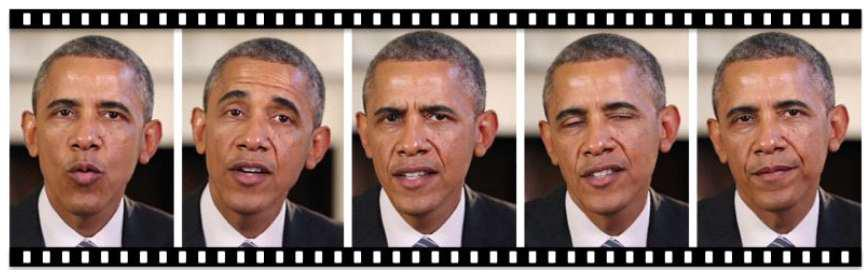
\includegraphics[scale = 0.5]{pic/chp1/img612}
    \caption{  버락 오바마 전 미국 대통령의 가짜 영상 \protect\footnote{출처: 워싱턴대학교}}
\end{figure}


\item Unsupervised Image-to-Image Translation with Generative Adversarial Networks : 이 연구는 “image-to-image translation” 문제를 GAN을 활용하여 해결한 연구이다. 총 2가지에 대해 실험을 하였다. 1) Gender transformation 2) Face swapping 하지만 이 연구는 obama-Hillary 데이터셋에 한정된 실험을 하였으며, edge detection에 있어서 부족한 결과를 내었다.

\begin{figure}[h!]
    \centering
      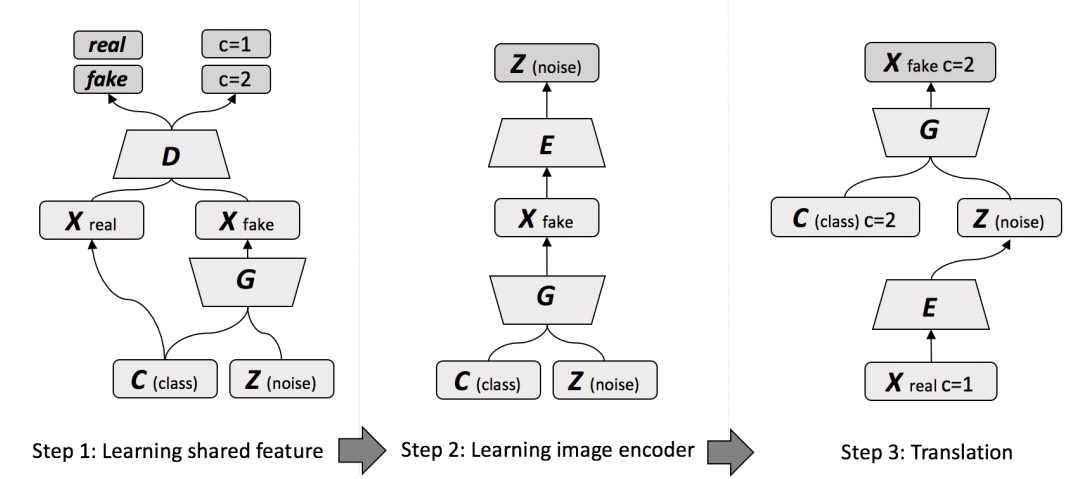
\includegraphics[scale = 0.7]{pic/chp1/img613}
    \caption{ GAN Architecture\cite{reference5}}
\end{figure}

\end{enumerate}

\subsection{얼굴교체 기술의 문제점}
\begin{enumerate}
    \item technical model : 

    얼굴 검출 및 특징점 관련 기술에 대해서는 커다란 이슈가 없는 상황이면서 이미 사람의 수준을 뛰어넘어 더욱 향상되어질 상황만 남은 상태이다. 최근 중국이 1000만개의 데이터셋을 이용하여 세계 1위를 차지한 것이 화제가 되었다. 반면 얼굴 관련 알고리즘에 우수한 성적을 꾸준히 보여왔던 미국은 10위 안에 딱 1개의 팀만이 들어가 있었으며, 이에 연구자들은 기술적인 모델보다는 데이터셋에 대해 훨씬 많은 관심을 보였다. 따라서 향후 연구에서는 기술적인 모델은 가장 결과가 자연스러운 GAN을 활용한 연구를 벤치마킹(+응용)하여 가져다 쓰되, 데이터셋이나 하드웨어에 대한 깊은 고민이 있어야 할 것이다.

    \item data dependency : 

    앞서 말했듯이 연구자들은 중국이 세계 1위를 가볍게 탈환한 이유를 거대한 데이터의 존재로 예측하고 있다. 실제로 본 팀에서 GAN을 활용하여 한 실험에서도 데이터에 상당히 의존적인 것을 확인 할 수 있었다. 가령 Masking 방식이나 그 외의 방식 또한 그렇지만 GAN은 제일 영향을 많이 받는 모델이다. 예를 들어, A -> B로 얼굴을 변형하는 상황에서 A의 입주변에 마이크가 있다면 B에서의 얼굴 변형을 실행할때도 입주변에 마이크가 같이 생성되게 된다. 또한, 만족스런 결과를 얻기 위해선 상당수의 질이 좋은 데이터와 매우 긴 훈련 시간을 가져야 한다. 여기서 질이 좋은 데이터란 기본적으로 얼굴 근처에 장애물이 없는 이미지와 정면을 바라보고 있는 얼굴이 많을 수록 좋다는 뜻이다. 따라서 향후 연구에서는 데이터 수집 또는 수집이 불가할 경우 data augmentation을 통한 데이터 생성에 대한 연구가 함께 진행되어야 할 것이다.

    \begin{figure}[h!]
        \centering
          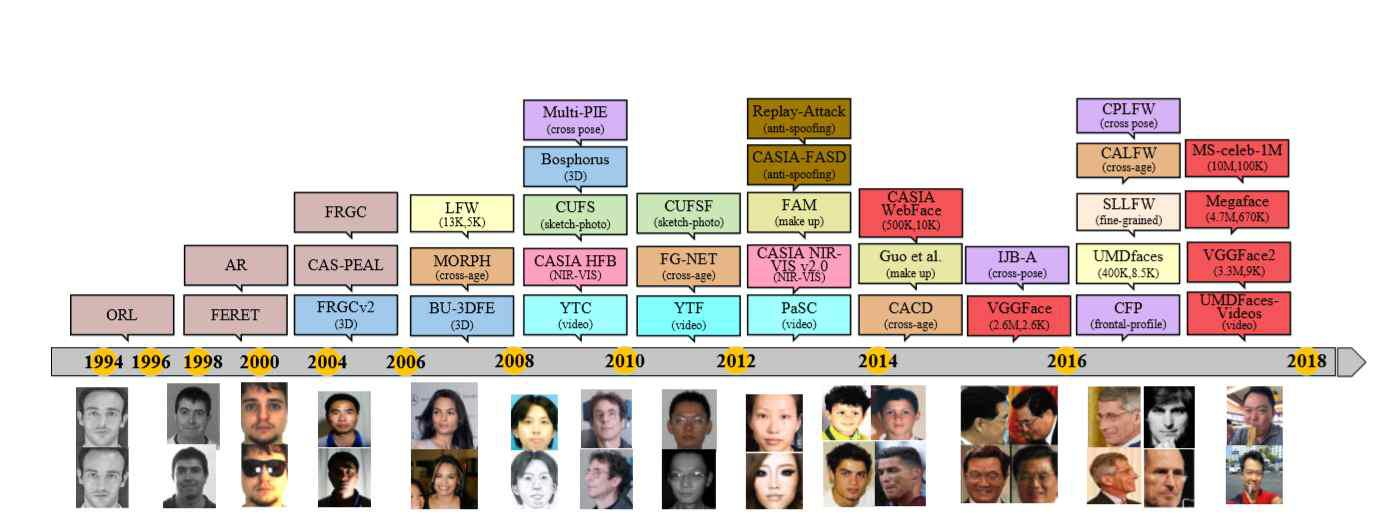
\includegraphics[scale = 0.8]{pic/chp1/img669}
        \caption{Face 연구용 데이터의 변화 \cite{reference6}}
    \end{figure}

    \item hardware dependency : 

    얼굴 관련 신경망 모델은 다른 문제 해결에 필요한 하드웨어 충족 조건보다 큰 조건을 요구한다. 왜냐하면 얼굴에서의 많은 굴곡에 대한 처리와 구체적인 특징 파악에 있어 많은 파라미터를 요구하기 때문이다. 또한, 세밀한 특징들을 잡기 위해선 신경망이 깊어질 필요가 있어 우수한 하드웨어 조건을 요구하게 될 수 밖에 없다. 물론 모델 깊이를 줄인다면 연구자의 하드웨어에 맞게 훈련을 시킬 수 있겠지만 그만큼 결과가 안좋아질 가능성이 높다. 따라서 향후 제품으로 사용될 경우엔 충분히 소비자가 납득할 만한 결과를 낼 수 있는 모델을 가동할 수 있는 하드웨어를 장착해야 할 것이다. 

    \item 연구의 시사점 : 

    현재 FR(Face Recognition)분야 관련해서는 학교 수준의 연구는 더 이상 진행하지 않아도 된다고 많은 연구자들이 평가하고 있다. 이미 공개되어진 VGGFace모델과 dataset을 사용하는 것이 다른 것보다 더 효율적일 것이다. 향후 ETRI에서는 COX에서의 기능 탑재를 위해 모델 관련 연구에 대한것 보다는 Dataset, Data-Preprocessing, Face DB 구축하는 방향의 연구를 진행해야 할 것이다. 또한, 최근 FR 연구 Issue중 하나인 모바일에서 처리가 가능한지에 대해서도 연구를 진행하여야 한다.
        
\end{enumerate}

%%%%%%%%%%%%%%%%%%%%%%%%%%%%%%%%%%%%%%%%%%%%%%%%%%%%%%%%%%%%%%%%%%5
\chapter{ 2D-Faceswap 모델의 기술 분석 및 구현 }

\section{2D-Faceswap 모델의 개요와 얼굴 합성 알고리즘 분석}

2D-faceswap 모델은 데이터 셋이 바꾸고자 하는 사진 1장으로 영상 데이터에 얼굴을 합성시키기 때문에 연산량이 적어 속도가 빨라 실시간으로 결과를 볼 수 있다. 

2D-faceswap 모델에서 쓰인 기술 중 CANDIDE라는 기술이 있는데 이 기술은 인간 얼굴의 모델 기반 코딩을 위해서 특별히 개발된 매개 변수화된 안면 마스크이다. Polygon의 수가 적으면 중간 정도의 컴퓨팅 성능으로 신속하게 재구성 할 수 있다.

얼굴을 인식할 때 68개의 랜드마크라 부르는 특정 포인트(턱의 상단, 눈 바깥의 눈꼬리부분, 눈썹 안쪽의 가장자리, 등)을 찾아낸다. 이 기술은 face landmark estimation[3]이라는 기술을 쓰는데 면 정렬을 밀리 초 단위로 수행하여 표준에 대한 최첨단 방식보다 우수하거나 비교할 수 있는 정확성을 제공한다. 

\begin{figure}[h!]
  \centering
    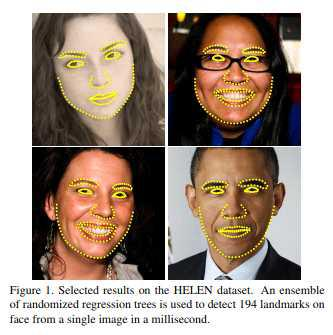
\includegraphics{pic/chp2/img684}
  \caption{\cite{reference7}}
\end{figure}



이 모델에서 쓰이는 기술 중 하나인 CANDIDE는 여러 개의 정점과 이를 이은 삼각형을 통해서 글로벌 및 로컬 작업 단위에 의해서 제어된다.


%%%%%%%%%%%%%%%%%%%%%%%%%%%%%%%%%%%%%%%%%%%%%%%%%%%%%%%%%%%%%%%%%%%%%%%%%%%%%%%%5
\begin{figure}[h!]
\centering
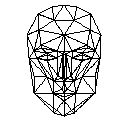
\includegraphics{pic/chp2/img690}
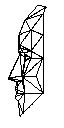
\includegraphics{pic/chp2/img693}
\caption{Candide-1}
\end{figure}
%%%%%%%%%%%%%%%%%%%%%%%%%%%%%%%%%%%%%%%%%%%%%%%%%%%%%%%%%%%%%%%%%%%%%%%%%%%%%%%%5

\begin{figure}[h!]
    \centering
    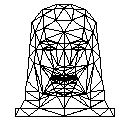
\includegraphics{pic/chp2/img694}
    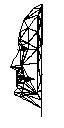
\includegraphics{pic/chp2/img695}
    \caption{Candide-2}
\end{figure}

\begin{figure}[h!]
    \centering
    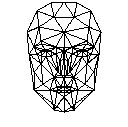
\includegraphics{pic/chp2/img696}
    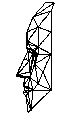
\includegraphics{pic/chp2/img697}
    \caption{Candide-3}
\end{figure}

이를 이용하여 얻어진 각 정점과 삼각형에 맞도록 2D 이미지 데이터를 3D 이미지 데이터로 변환시켜 학습된 모델을 통하여 fitting 시키게 되면 각 프레임 별로 결과가 나오는 것이다.

2D 이미지 데이터에서 3D 데이터로 변환시키는 과정은 [8]의 논문을 보면 알 수 있는데 
얼굴 공간 내의 각 속성에 대한 표본면의 분포를 평가하여 ‘후크 된’ 코 또는 사람의 가중치를 측정하여 거의 모든 얼굴을 생성 할 수 있는 파라미터의 얼굴 모델의 구성한 후, 대응되는 문제는 수학적 최적화의 문제로 변환 시킨다. 이를 통해 3D 얼굴을 얻을 수 있다.

마지막으로 색상을 교정한 뒤 결과물을 얻어낼 수 있다.

\begin{figure}[h!]
  \centering
    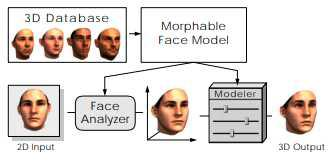
\includegraphics{pic/chp2/img712}
  \caption{ 3D morphable model image\cite{reference7}}
\end{figure}


\section{2D-Faceswap 모델의 분석}

알고리즘 과정을 살펴보면 먼저 입력 이미지를 가져와서 얼굴 영역과 그 경계표를 찾아낸다. 그 후 3D 모델을 랜드 마크에 맞춰 이미지에 투영된 모델의 정해진 점이 텍스처의 좌표가 된다. 이 것들이 완료되면 모든 것이 초기화되고 카메라가 이미지 캡처를 시작한다.(동영상의 경우 프레임을 뽑아낸다.) 캡처된 각 이미지에 대해서 다음 단계가 수행된다.

\begin{enumerate}
    \item 얼굴 영역이 감지되고 얼굴의 표식이 배치된다.
    \item 3D 모델은 위치가 지정된 랜드마크가 fitting 된다.
    \item 3D 모델은 초기화하는 동안 얻은 텍스처와 함께 렌더링된다.
    \item 렌더링 된 모델의 이미지는 간단한 색상 교정을 사용하여 카메라에서 얻은 이미지(동영상의 경우 뽑아낸 프레임) 와 혼합된다.
    \item 최종 이미지가 사용자에게 표시된다.
\end{enumerate}

이 전체 프로세스에서 가장 중요한 요소는 3D 모델의 피팅이다. 

3D 모델 자체의 구성은 다음과 같다.

\begin{itemize}
    \item 중립면 모델의 3D 모양.
    \item 입 열기, 눈썹 올리기 등을 만들기 위해 중립면에 추가 할 수 있는 여러가지 블렌딩 쉐이프, 얼굴의 삼각형으로 형성된 얼굴 모양의 인덱스 삼중 세트.
    \item 랜드마크 로컬 라이저에 의해 발견된 표식과 3D 얼굴 형태의 정점 사이에서 일치를 설정하는 두 세트의 인덱스.
    \item 모델은 다음의 방정식을 통해서 이미지에 투영된다.
    \[ s = aP \left( S_{0} + \sum_{i=1}^{n} w_{i}\cdot S_{i}  \right)   \]

    여기서 $s$는 투영된 모양, $a$는 배율의 매개변수, $P$는 3D 모양을 회전시키는 회전 행렬의 처음 두 행, $S_0$는 중립면의 모양, $w_i$은 블렌드 모양의 가중치, $S_i$은 블렌드 쉐이프, $t$는 2D 변환 벡터, $n$은 블렌드 쉐이프의 수이다.
    모델 피팅은 투영된 모양과 랜드마크 간의 차이를 최소화하여 진행된다. 모양과 랜드마크의 차이의 최소화는 Gauss Newton방법을 이용하여 블렌드 형태의 가중치, 스케일링, 회전 및 평행 이동 등 다양한 변환을 수행한다.\cite{reference9}
\end{itemize}

\section{2D-Faceswap 모델의 테스트 환경 및 결과}

\subsection{테스트 환경}
\spec
\subsection{결과}

데이터 셋이 1개면 되기 때문에 deep learning을 이용한 방법과 달리 계산량이 적어서 실시간으로 변 환이 가능하며 결과를 바로 볼 수 있다. 그리고 정면영상의 경우 상대적으로 짧은 시간에 좋은 결과 를 볼 수 있다.

실시간으로 소통이라는 경험을 원하는 사람은 이를 통한 방법으로 faceswap을 지원하면 될 것이다.  하지만 데이터 셋이 1개이며 이를 통한 정점 추출과 3D modeling은 다양한 각도에서 많은 양의 데이 터를 사용하는 deep learning 모델과는 결과물의 퀄리티 차이가 심하다. 일부 화면에서는 심하게 노이 즈가 발생하는 경우도 있고 얼굴인식을 정확하게 하지 못하는 경우 합성 자체가 아예 실행되지 않는 다.

결과사진 

\begin{figure}[h!]
  \centering
    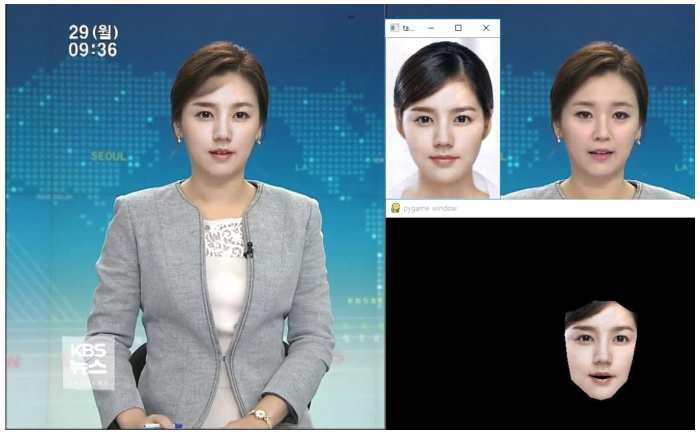
\includegraphics{pic/chp2/img747}
  \caption{ 3D morphable model image\cite{reference7}}
\end{figure}



\chapter{Openpose를 활용한 Faceswap 모델의 기술 분석 및 구현}

\section{Openpose를 활용한 모델의 개요와 얼굴 합성 알고리즘 분석}

Openpose는 고가의 센서 장비가 필요한 기존의 모델들과는 달리 일반 카메라를 통해서도 사람 인체의 스켈레톤 데이터를 태깅할 수 있는 딥 러닝 네트워크이다. 키넥트와 같은 고가의 장비들이 없이도 일반 카메라를 통해 스켈레톤 태깅이 가능하며 그 결과는 매우 좋다.
%%%%%%%%%%%%%%%%%%%%%%%%%%%%%%%%%%%%%%%%%%%%%%%%%%%%%%%%%%%%%%%%%%%%%%%%%%%%%%%%5
\begin{figure}[h!]
\centering
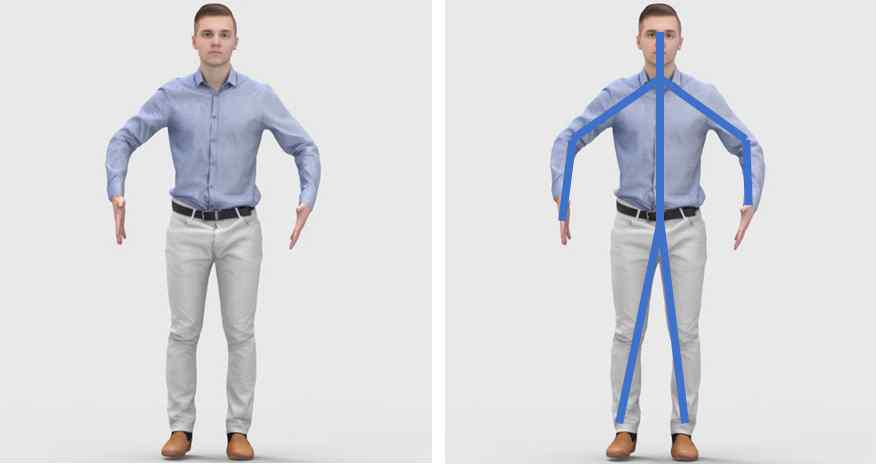
\includegraphics{pic/chp3/img761}
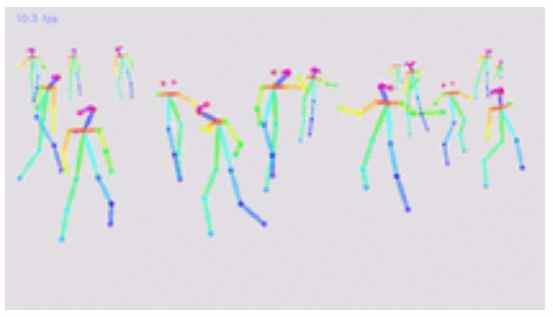
\includegraphics{pic/chp3/img762}
\caption{태깅 된 인체 스켈레톤 데이터}
\end{figure}
%%%%%%%%%%%%%%%%%%%%%%%%%%%%%%%%%%%%%%%%%%%%%%%%%%%%%%%%%%%%%%%%%%%%%%%%%%%%%%%%5
\begin{figure}[h!]
  \centering
    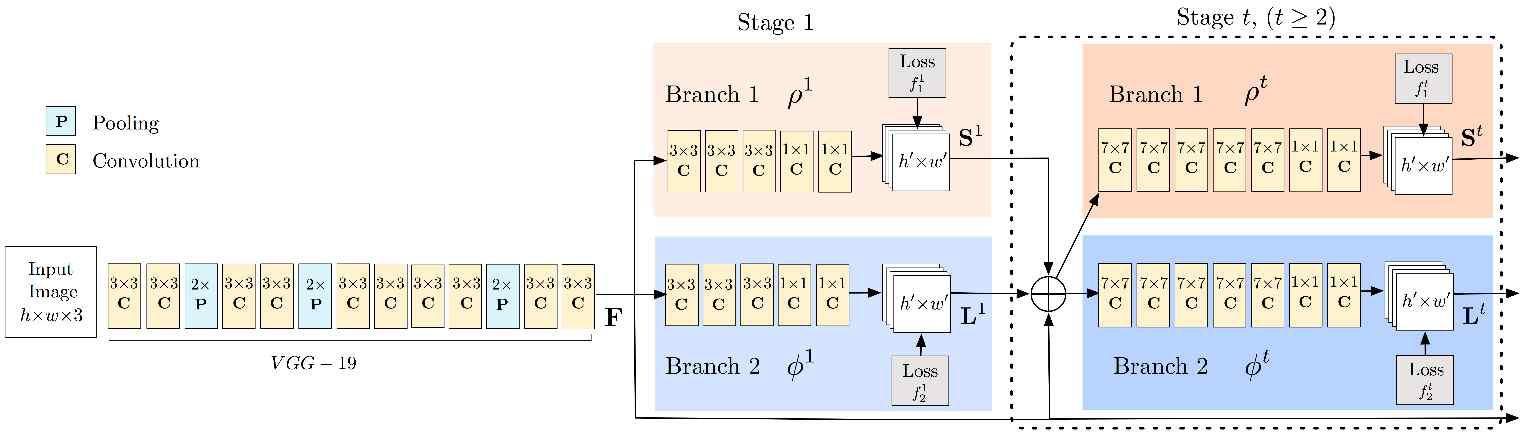
\includegraphics[scale = 0.5]{pic/chp3/img763}
  \caption{Openpose의 네트워크 구조\cite{reference10}}
\end{figure}


Openpose의 네트워크 구조를 보면 vgg-19 네트워크를 차용하여 모델을 구현하였으며 입력 이미지 데이터가 vgg-19 네트워크를 통과하면 이미지의 feature가 강조된 형태로 출력된다. 출력된 데이터는 Stage 1부터 Stage 6까지의 입력데이터로 다시 이용되어 최종 결과가 출력된다.

vgg-19 네트워크를 통과한 후 Stage 1 ~ Stage 6에서는 실제 정답인 Ground-truth와 네트워크가 도출한 정답과의 비교를 통해 모델의 loss값을 구하고 이를 최적화해 나가는 방향으로 모델을 학습해나간다.

\begin{figure}[h!]
  \centering
    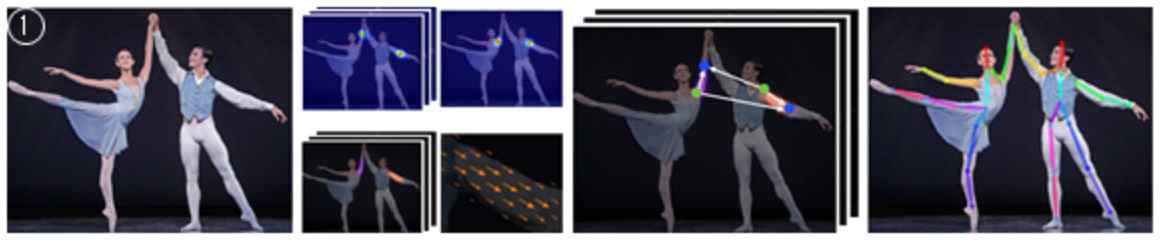
\includegraphics[scale = 0.7]{pic/chp3/img765}
  \caption{Openpose의 학습 과정\cite{reference10}}
\end{figure}


입력 이미지가 vgg-19 네트워크를 통과하게 되면 28x28x512의 크기로 feature가 강조된 데이터를 얻을 수 있으며 해당 데이터를 각 Stage의 입력데이터로 사용한다. 각 스테이지에서는 입력데이터를 받게 되면 2개의 branch를 통해 각각 confidence map과 affinity field를 구하게 된다. Confidence map은 이미지 속 사람의 관절 위치를 파악하는데 사용되며 Affinity field는 이미지에서 추출된 스켈레톤의 주인이 누구인가 파악하는데 사용된다.

vgg-19 네트워크를 통과한 후 얻은 feature 데이터는 초기에 큰 의미가 없는 데이터이다. feature 데이터를 human pose 데이터와 비교를 하면서 점점 그 차이를 줄여나가는 방향으로 모델의 최적화를 진행하게 되면 큰 의미가 없었던 feature들은 점점 사람의 관절 위치를 가르키는 Confidence map을 나타나게 될 것이다.

Affinity field 학습의 경우 각 관절의 주인이 누구인가를 파악하기 위하여 각 부분의 운동 방향에 대한 데이터가 필요로 한다. 모델 학습을 위한 데이터셋은 크게 COCO 데이터셋과 MPII 데이터셋을 사용할 수 있다.

학습이 완료되면 confidence map과 affinity field를 조합하여 완성된 인간 스켈레톤을 생성해야 한다.

Openpose는 인체의 스켈레톤을 태깅함과 동시에 얼굴 부분 70개의 특징점 또한 도출 한다. 이 70개의 얼굴 특징점을 이용하여 얼굴 변형 모델을 구현할 수 있다.

[제 2 장]에서 제시한 얼굴 변형 모델을 Openpose과 결합하여 새 모델을 제안할 수 있다. 앞서 제시한 모델에서는 68개의 얼굴 특징점을 찾고 해당 특징점을 이용하여 얼굴 변형 알고리즘을 진행하게 된다. Openpose를 통해 인간의 신체구조를 파악하고 그 중 얼굴의 위치와 70개의 얼굴 특징점을 이용하여 [제 2 장]에서 제시한 모델을 발전시킬 수 있다. 70개의 얼굴 특징점을 활용하여 3D로 렌더링한 후 3D 좌표점을 만들어내고 이를 기반으로 3D Mask를 생성하여 [제 2 장]에서 제시한 모델과 동일한 방향으로 얼굴 변형을 진행하게 된다.

Openpose를 앞선 모델에 추가함으로써 얼굴 변형에 더 많은 70개의 얼굴 특징점을 이용하게 된다. 이를 통해 비교적 유연하고 자연스러운 얼굴 변형을 할 수 있다. 또한 속도가 검증된 Openpose 모델을 이용함으로써 실시간 얼굴 변형에 유리하다. 신체 움직임이 활발한 동영상의 얼굴 변형을 시도할 경우 이전 모델보다 더 높은 성능을 기대할 수 있다.

\section{Openpose를 활용한 얼굴 변형 모델의 테스트 환경 및 결과}

\subsection{테스트 환경}
\spec
\subsection{ 결과 }

학습된 Openpose를 활용한 얼굴 변형 모델을 테스트한 결과는 다음과 같다.
%%%%%%%%%%%%%%%%%%%%%%%%%%%%%%%%%%%%%%%%%%%%%%%%%%%%%%%%%%%%%%%%%%%%%%%%%%%%%%%%5
\begin{figure}[h!]
  \centering
        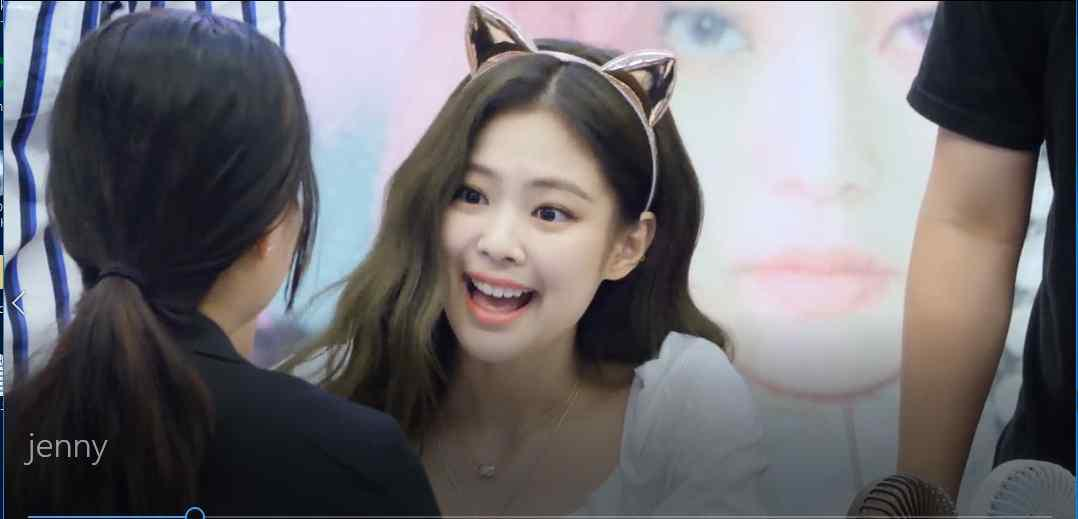
\includegraphics{pic/chp3/img778}
        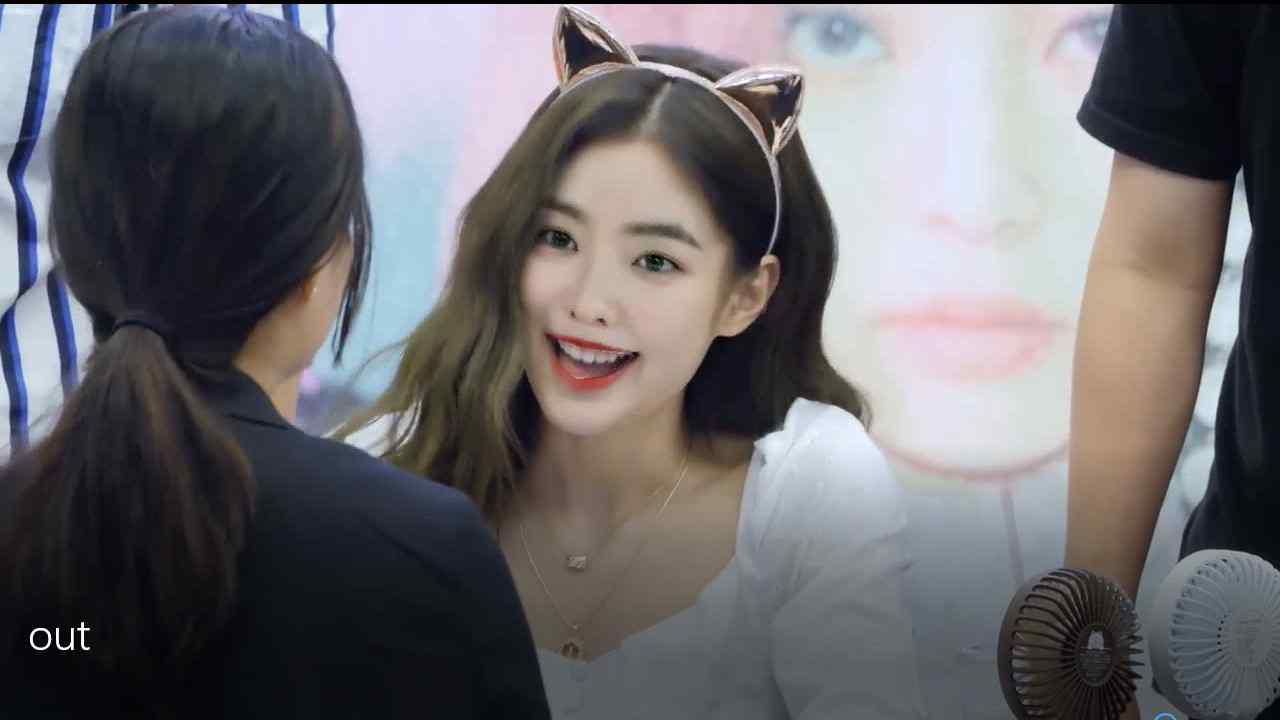
\includegraphics{pic/chp3/img779}
  \caption{원 이미지(위), 얼굴 변형 된 이미지(아래)}
\end{figure}
%%%%%%%%%%%%%%%%%%%%%%%%%%%%%%%%%%%%%%%%%%%%%%%%%%%%%%%%%%%%%%%%%%%%%%%%%%%%%%%%5


이 모델을 이용하여 [제 2 장]에서 제시한 모델에 비해 더 빠르게 실시간 얼굴 변형이 가능하며, 더 많은 얼굴 특징점으로 인해 생성된 Mask가 좀 더 명확하고 유연하게 되었다. 하지만, 눈, 코, 입 부분에서의 불안정한 변형과 학습 시 다양한 데이터를 사용하지 않는다는 점은 이 모델의 한계점이 될 수 있다.

\chapter{딥페이크(Original-High-Resolution Model)의 기술 분석 및 구현}

\section{ 딥페이크의 개요와 얼굴 합성 알고리즘 분석}

딥페이크란 인공지능을 이용하여 영상에 얼굴을 합성시킬 수 있는 기술이다. 미국 커뮤니티사이트 레딧에서 deepfakes는 이름의 유저가 TensorFlow같은 오픈소스 소프트웨어를 이용하여 유명연예인과 포르노를 합성한 것이 이 기술의 시작이다.

우리가 이용한 \cite{reference11} 깃허브의 소스코드에는 여러가지 모델들이 들어있는데 그 중 오토인코더를 사용한 Original-High-Res 모델을 사용하여 실험을 진행했다.

딥페이크의 얼굴 합성 과정은 가장 먼저 학습시키고자 하는 데이터 셋을 준비하여 얼굴을 인지한다. 이 얼굴인지 과정의 기술은 dlib-HOG, dlib-CNN이 쓰인다. 그 후 얼굴 피처를 따로 추출한다. 이후 인코딩이 쉽도록하기 위한 얼굴정렬과정을 거친다. 인코딩 단계에서 얼굴의 특징점 예를 들면 눈, 코, 입, 등의 부분들을 Deep Convolutional Neural Network(딥 컨볼루션 신경망)을 이용하여 학습시킨 뒤 얼굴을 적절하게 잘라내고 적절한 블러와 샤프닝 등 추가 가공을 하여 얼굴을 합성한다.


\begin{figure}[h!]
\centering
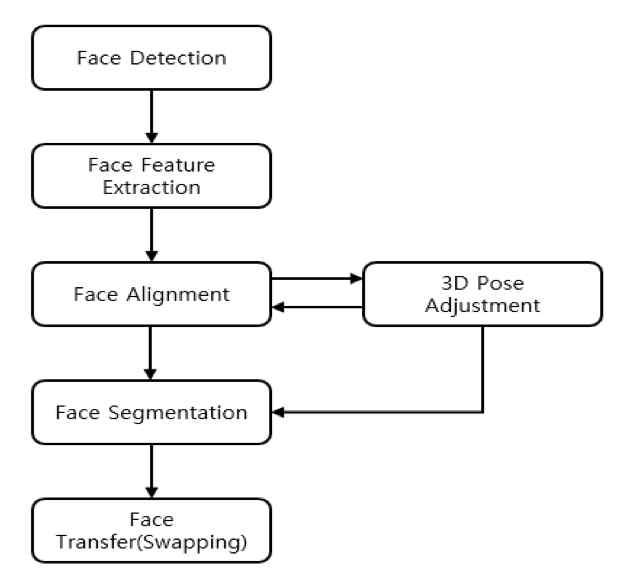
\includegraphics{pic/chp4/img798}
\end{figure}


\section{ 딥페이크 내의 모델 분석}

딥페이크는 인공지능 기반의 기술로서 내부에서 사용한 모델은 오토인코더를 사용하였다. 오토인코더란 출력값을 입력값의 근사로 하는 함수로 학습을 진행하는 비지도 학습이다. 데이터의 처리과정은 인코딩 과정을 통해서 히든 레이어로 이동하고 다시 디코딩 과정을 통해서 출력값을 가지게 된다.

인코딩을 거치게 되면 정보들 중 핵심적인 정보들이 걸러지게 되는데 이를 피처라고 한다. 피처를 다시 디코딩을 통해서 입력과 최대한 비슷하도록 출력한다.

\begin{figure}[h!]
\centering
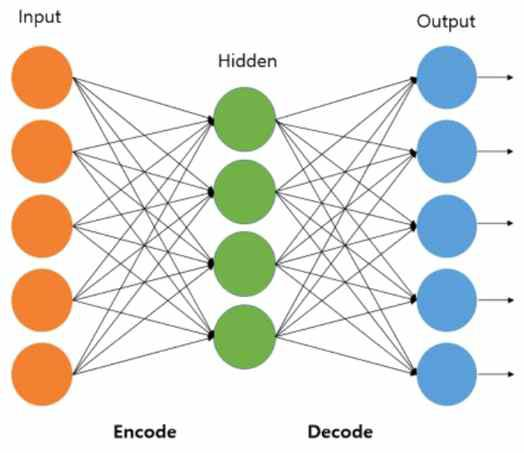
\includegraphics{pic/chp4/img802}

\end{figure}

합성 결과가 잘 나오려면 데이터가 중요하기도 하지만 모델의 학습이 올바르게 진행되고 적절한 시점에서 학습을 중단시켜야 한다.

이를 판단하는 척도로서 에러의 절대값 평균을 이용한다. 입력한 데이터의 결과값으로 아웃풋 데이터가 나오면 이를 절대값 평균을 이용하여 바꾸고자 하는 얼굴과 얼마나 다른지를 나타낼 수 있다. 또한 활성화 함수로 ReLU함수를 사용하고 있고 이를 사용하는 이유는 역전파를 잘 시키기 위함이다. 특히 ReLU함수는 기존의 많이 쓰이던 sigmoid function의 Gradient Vanishing 문제를 해결하기 위해 최근에 많이 사용되고 있는 활성화 함수 중 하나이다.

역전파시 출력에서부터 입력과정에서 넘어온 데이터를 비교하여 틀린 정도를 미분한 값을 전달하게 되는데 기존 sigmoid fuction을 쓰게 되면 양 끝. 단에 기울기가 0에 가까워서 내가 원하는 값과 모양이 동 떨어지게 된다. 즉 underfitting이 일어나게 된다.

이 현상이 Gradient Vanishing 문제이다. 하지만 ReLU(Rectified Linear Units) 함수는 양의 구간에서 미분 값이 항상 1이기 때문에 역전파시에 출력값에서 입력값까지 미분값이 사라지지 않는다.

이 과정 이후 Loss fuction 즉 위에서 설명한 에러의 절대값 평균을 이용하는 것이다. 이 과정을 통하여 데이터의 가중치가 셋팅되고 가중치를 개선 시키는 과정에서 학습이 되는 것이다. 개선과정의 알고리즘으로 많은 아이디어들이 제시되고 있는데 현재 가장 유명한 알고리즘은 ADAM(Adaptive Moment Estimation)으로 알려져 있다. 실제로 현재 이용한 코드에서도 optimizer로 ADAM을 이용하고 있다.

ADAM이란 기존의 최적화 알고리즘의 아이디어가 발전과 개선으로 새로운 알고리즘이 제시되는데 이 알고리즘은 RMSProp과 Momentum 방식을 합친 것 같은 알고리즘이다.

최적화 알고리즘의 발전과정을 살펴보면 GD(모든 자료를 다 검토해서 최적의 방향과 스텝사이즈를 찾는다.) SGD(일부만 보고 빠르게 판단하여 방향과 스텝사이즈를 찾는다.) 여기서 스텝사이즈를 개선한 알고리즘은 Adagrad(살펴본 데이터는 빠르게 훑고 안 살펴본 데이터는 스텝사이즈를 줄여 세밀하게 살펴본다.) RMSProp(스텝사이즈를 줄이는 것은 좋지만 이전 맥락을 살펴보고 줄임) 그리고 방향을 개선한 알고리즘은 Momentum(움직인 방향의 관성방향을 주로 살펴본다.) 이후 나온 알고리즘이 ADAM이다.[12]

\begin{figure}[h!]
\centering
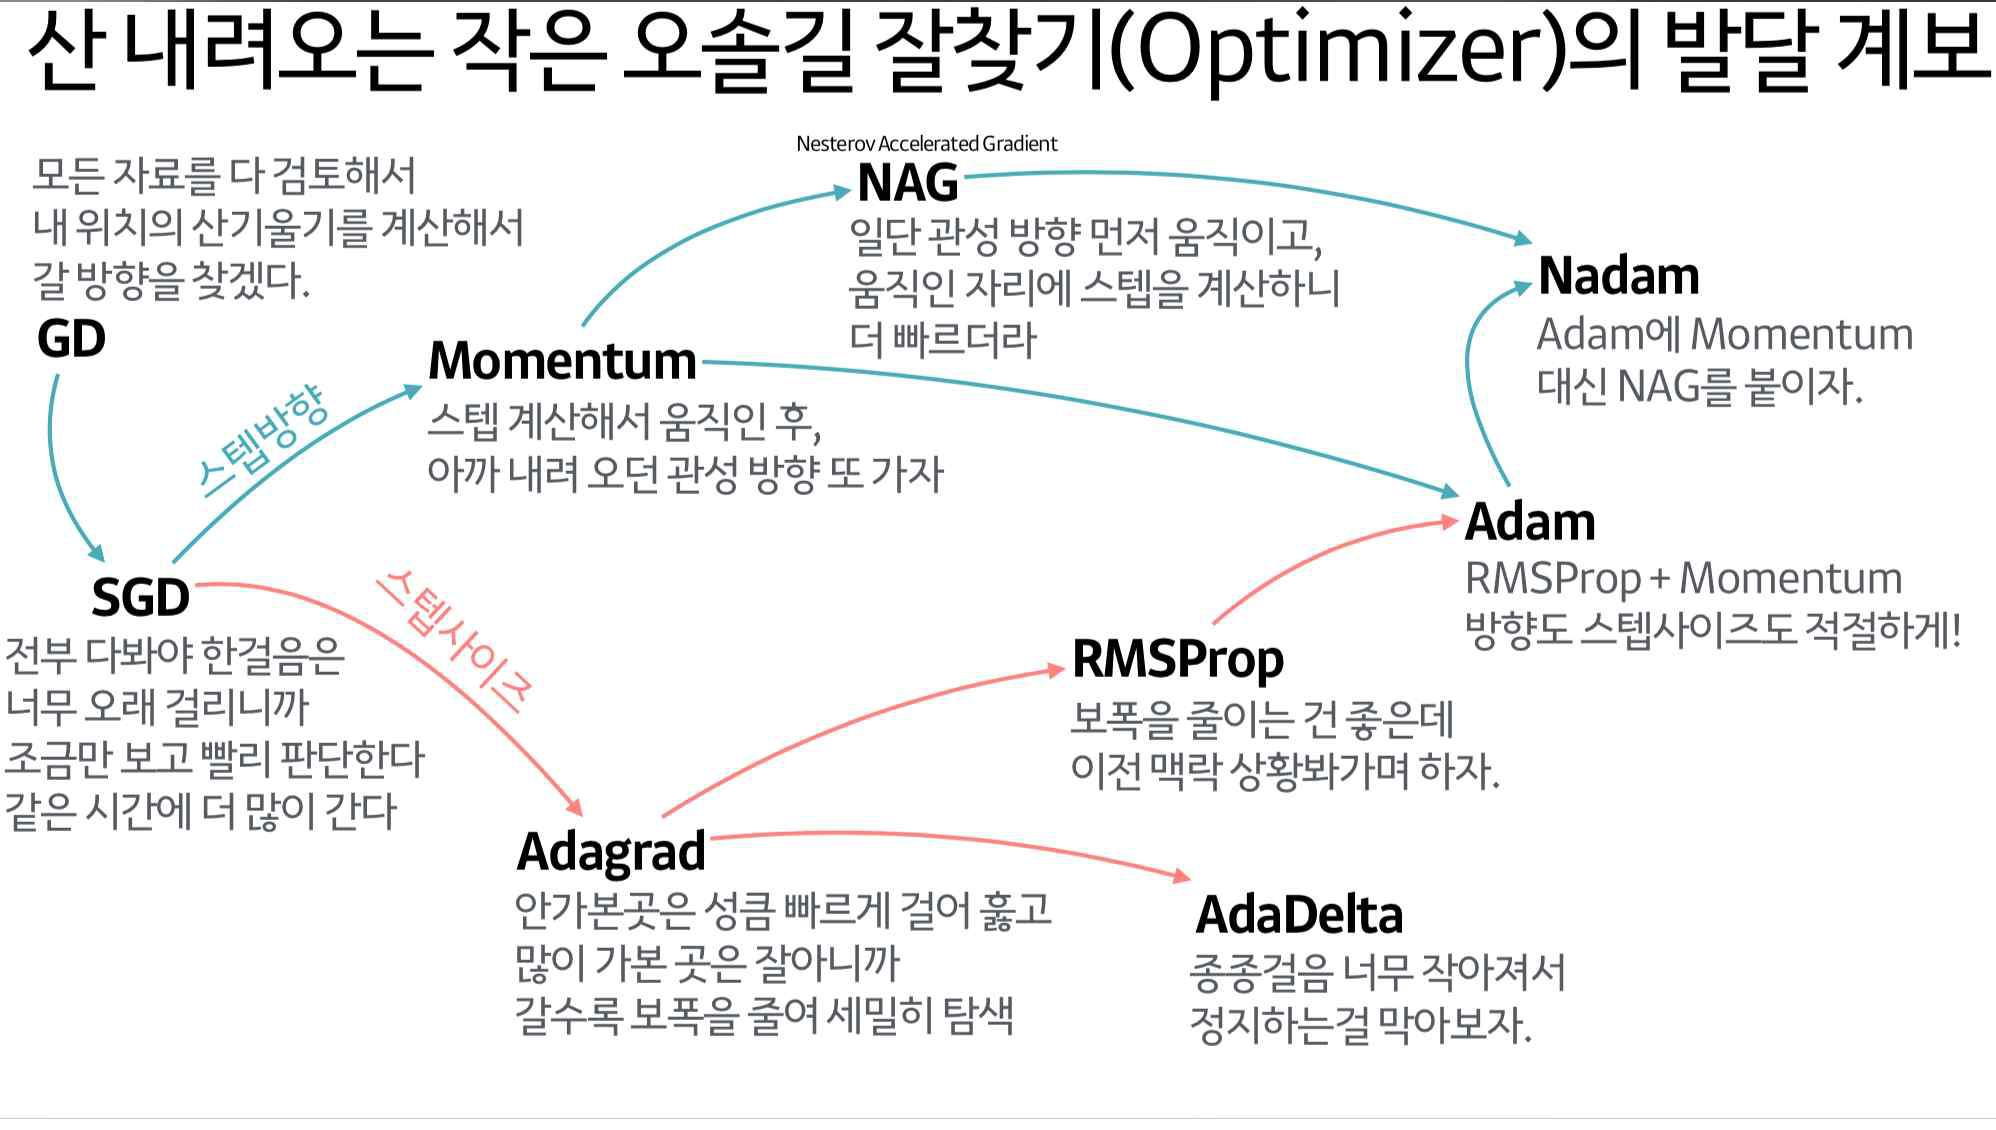
\includegraphics{pic/chp4/img825}
\end{figure}

또 한 가지 주의사항으로 학습 시 underfitting도 주의해야하지만 overfitting도 주의해야한다. 뉴럴넷에게 학습 시 융통성을 주기 위해서 Dropout 방법이 있다. Dropout은 학습 시 일부 노드를 제외시킴으로써 overfitting을 예방할 수 있다.

\begin{figure}[h!]
\centering
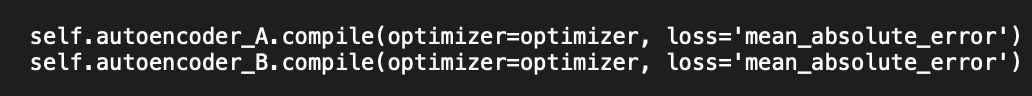
\includegraphics{pic/chp4/img831}
\end{figure}

\begin{figure}[h!]
\centering
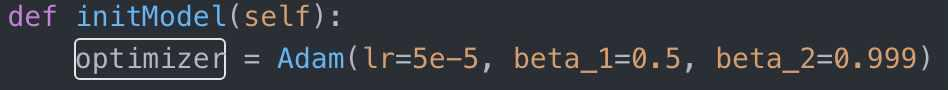
\includegraphics[scale = 0.7]{pic/chp4/img838}
\end{figure}

\section{ 딥페이크 모델의 테스트 환경 및 결과}

\subsection{테스트 환경 }
\spec
\subsection{결과}

본 프로그램을 통해 학습을 하고 얼굴을 합성하는 것은 위에서 연구한 2D-faceswap 모델과  openpose 모델과는 다르게 학습을 미리 실행하고 얼굴을 합성한다는 점에서 실시간으로 반응하기 어 렵다는 점이 있다. 즉 결과를 실시간으로 확인하기 어려우므로 결과를 확인하고 수정한 것을 반영하 는데 오랜 시간이 걸린다. 합성의 측면에서는 정면과 좌우 15도 정도의 각도에서는 상당히 자연스러 운 합성을 보여줬으며 고개를 아래로 숙이거나 위로 들어올리는 경우, 얼굴이 장애물로 인해 일정부 분 가려진 경우에는 합성이 이루어지지 않은 점이 한계라고 볼 수 있다.

결과사진 :

\begin{figure}[h!]
\centering
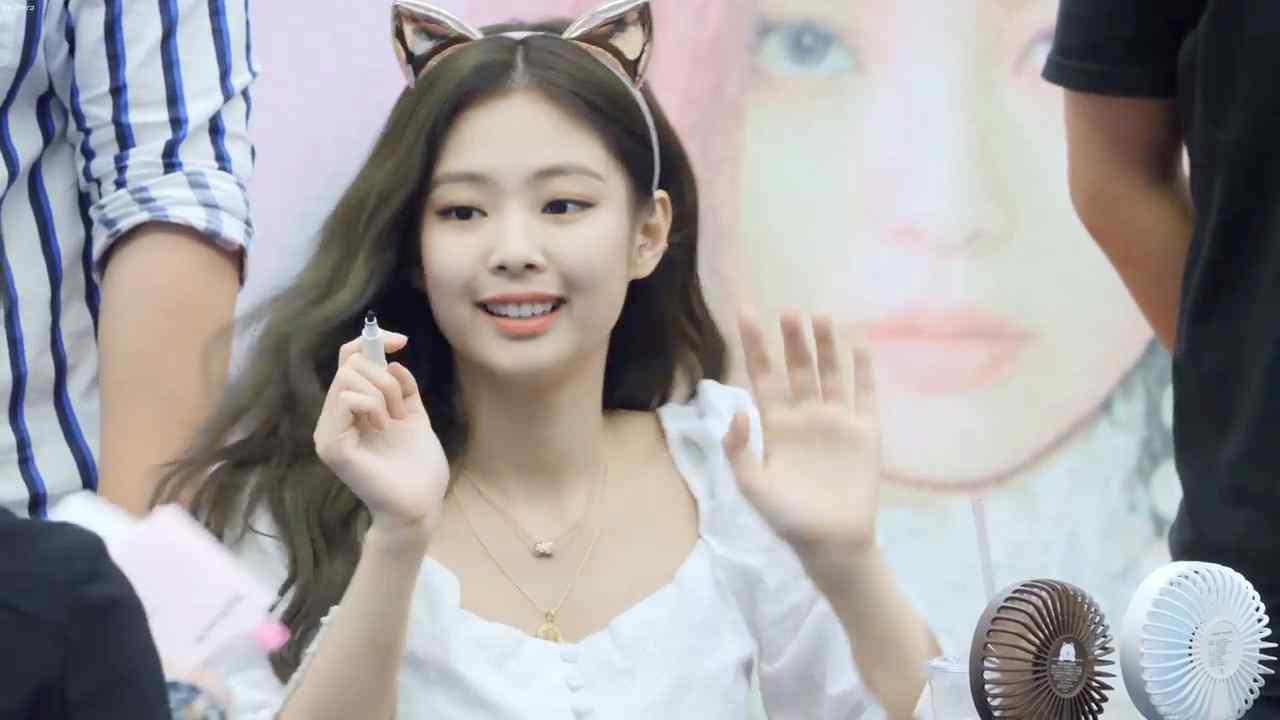
\includegraphics[scale = 0.5]{pic/chp4/img845}
\end{figure}

\begin{figure}[h!]
\centering
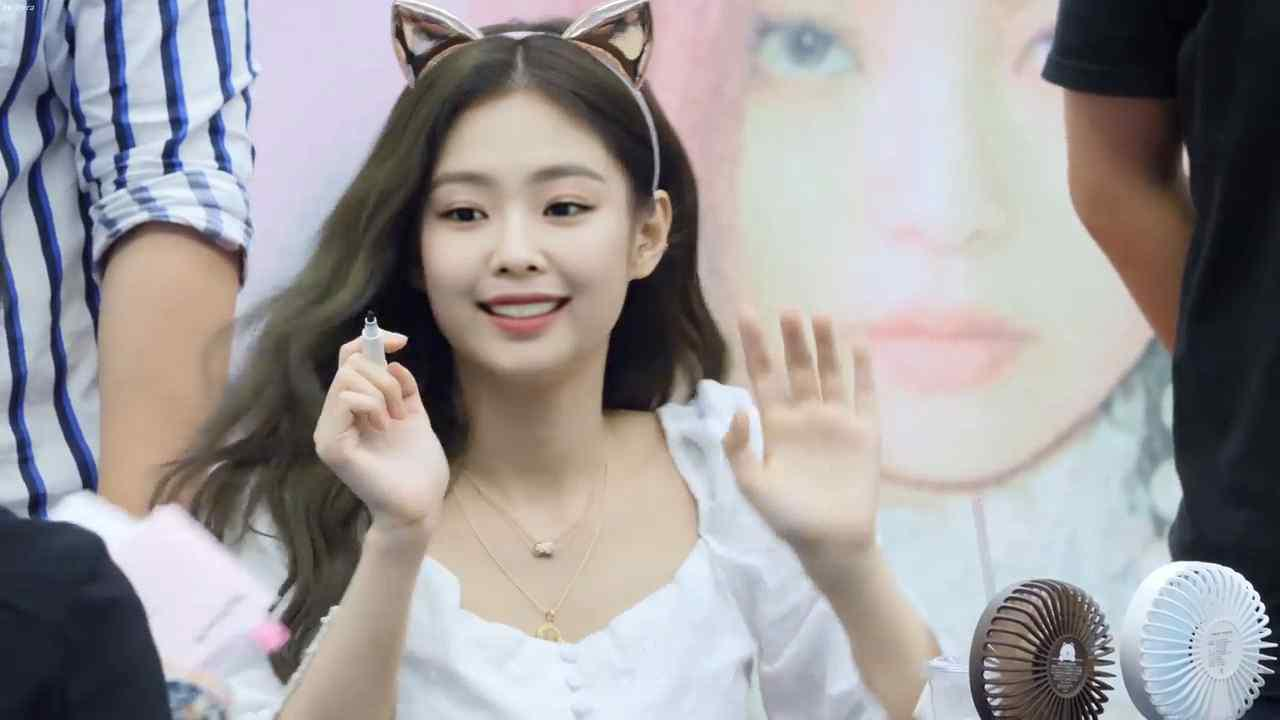
\includegraphics[scale = 0.5]{pic/chp4/img846}
\end{figure}

\chapter{ 생성적 적대 신경망(GAN)을 활용한 Faceswap 모델의 기술 분석 및 구현}


\section{ GAN을 활용한 얼굴 변형 모델의 개요와 얼굴 합성 알고리즘 분석}
2014년 'Ian Goodfellow'가 NIPS 학회에서 생성적 적대 신경망인 GAN(Generative Adversarial Nets)을 발표하면서 지도 학습 중심이었던 딥러닝의 패러다임이 비지도 학습으로 바뀌었다. 이후 많은 후속연구과 GAN을 이용한 사례들이 나타나고 있다. 기존 대부분의 인공지능 연구는 사람이 정답을 알려주는 방식인 지도 학습 방식으로 이루어져왔다. 따라서 지도 학습 방식은 학습이 가능하도록 데이터를 가공하는 수작업 과정이 필요하다. 하지만 비지도 학습 방식인 GAN은 인간의 개입이 없이 스스로 두 모델의 경쟁 과정을 거치면서 학습한다. 따라서 대량의 데이터를 가공해야하는 지도 학습 방식의 한계를 극복할 수 있다.

GAN은 두 모델 ‘생성자(G)’와 ‘구분자(D)’의 경쟁을 통해 학습을 진행하고 결과를 만들어낸다. '생성자‘는 데이터를 학습하여 학습에 사용된 데이터의 확률분포를 이용하여 가짜 데이터를 생성하는 것을 목표로 하며 실제에 가까운 가짜 데이터를 생성하도록 학습된다. ’구분자‘는 ’생성자‘가 생성한 가짜 데이터가 실제인지 가짜인지 구분하도록 학습된다.

GAN은 데이터가 이루는 확률분포를 예측하여 신경망을 통해 해당 데이터의 확률분포를 재현해 낼 수 있도록 학습된다. 이 과정에서 확률분포가 실제와 동일, 유사한가 또는 다른가를 ‘구분자’가 판단하게 된다. GAN의 ‘생성자’는 ‘구분자’가 점점 판단을 하기 어렵도록 분포를 생성할 수 있게 학습되는데 ‘구분자’가 판단하기 가장 힘든, 어느 쪽에도 치우지지 않은 0.5 확률로 진짜와 가짜가 구분될 수 있게 생성하도록 ‘생성자’가 학습된다. 이렇게 ‘생성자’는 ‘구분자’가 잘 구분할 수 없도록 생성하고, ‘구분자’는 ‘생성자’가 생성한 데이터의 진위 여부를 잘 판단하도록 적대적(Adversarial)으로 학습 하게 된다.

\begin{figure}[h!]
  \centering
    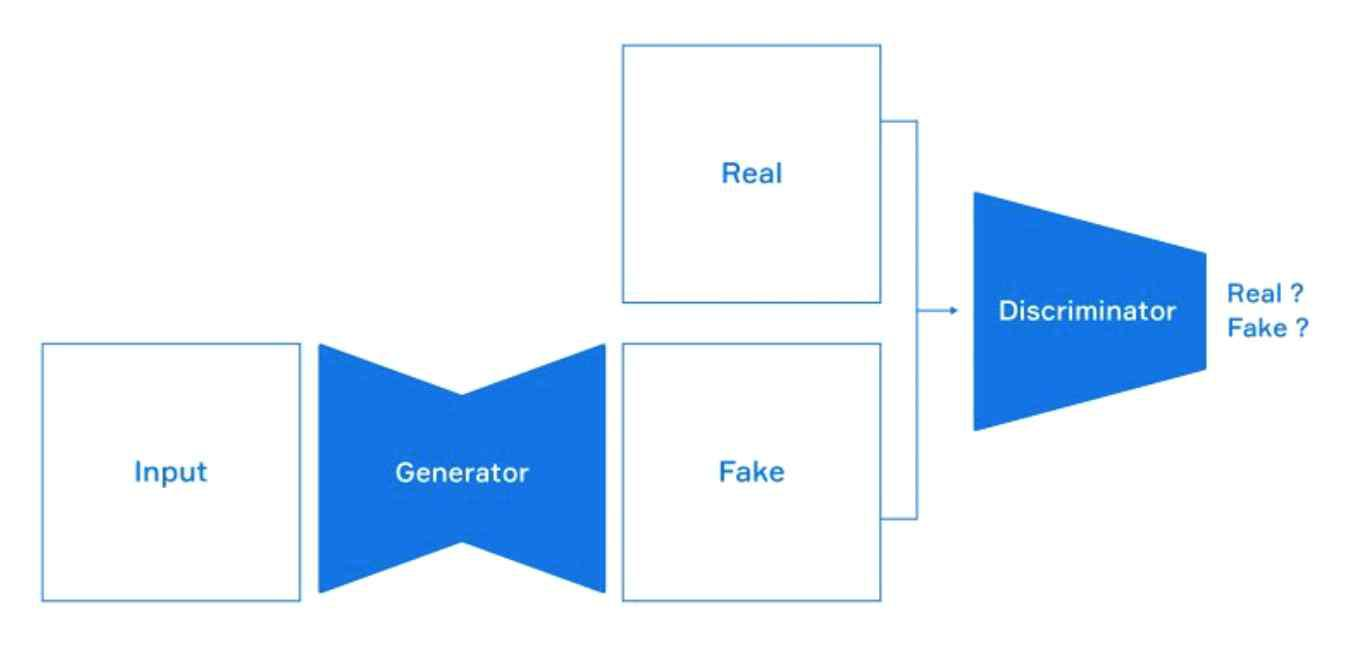
\includegraphics{pic/chp5/img858}
  \caption{GAN의 학습 과정 \protect\footnote{출처:네이버랩스}}
\end{figure}



GAN은 주로 이미지 생성에 활용되며 일반적인 경우 실제의 이미지를 학습해여 가짜 이미지를 생성해 내도록한다. 유명인들의 사진을 생성해내거나 유명화가의 그림을 생성해 내는 연구들이 진행되어왔다.

\begin{figure}[h!]
  \centering
    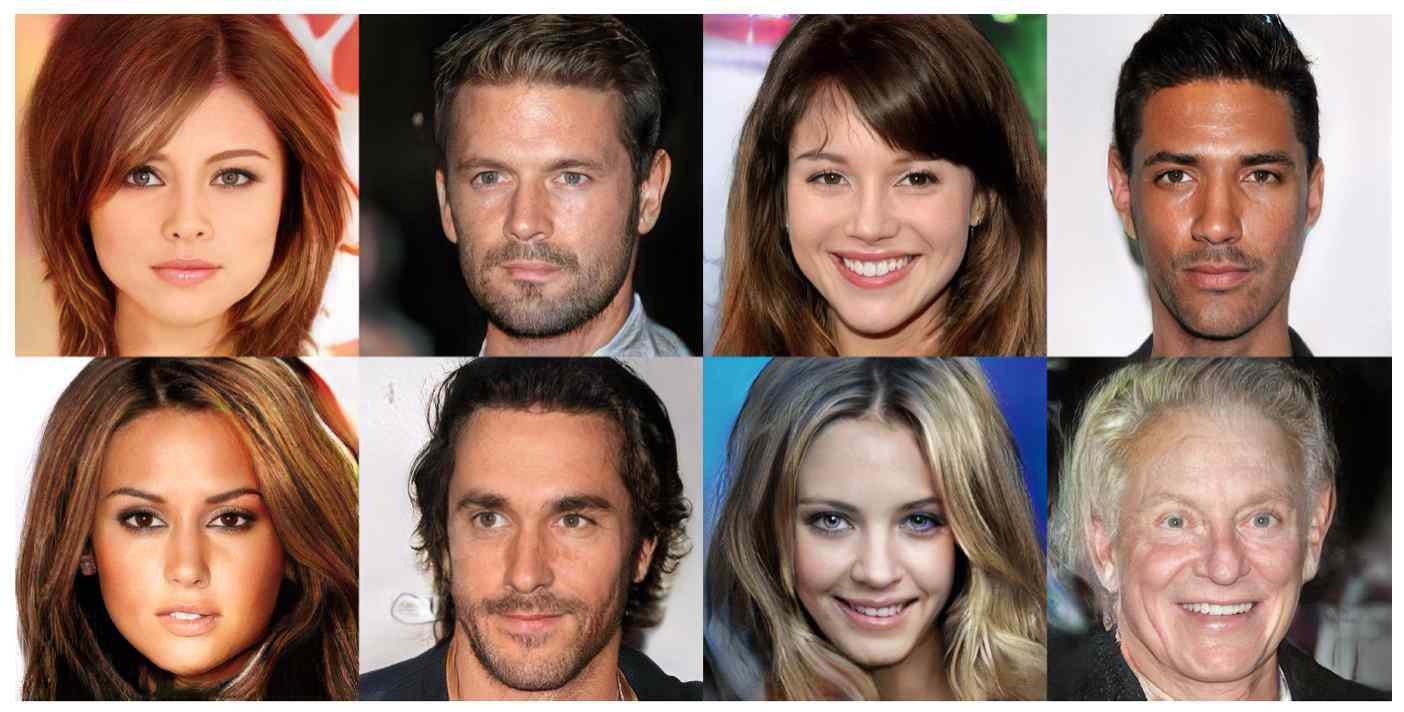
\includegraphics{pic/chp5/img866}
  \caption{GAN을 통해 유명인 사진을 바탕으로 만들어진 허구의 인물 \protect\footnote{출처:엔비디아}}
\end{figure}


\begin{figure}[h!]
  \centering
    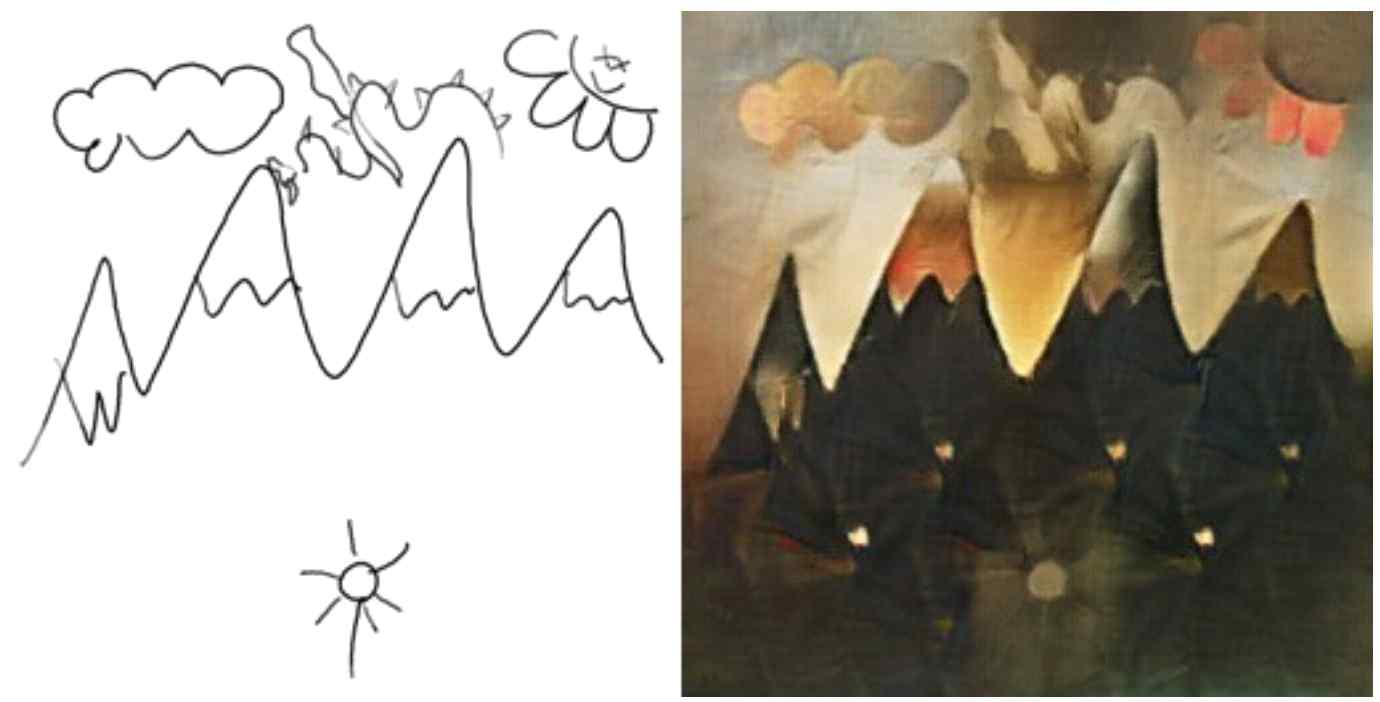
\includegraphics{pic/chp5/img868}
  \caption{반 고흐의 그림을 생성해 내는 빈센트 AI \protect\footnote{출처:엔비디아}}
\end{figure}


\section{ GAN을 활용한 얼굴 변형 모델 분석}

GAN을 이용한 얼굴 변형 모델\cite{reference11}을 이용하였다.

이 모델에서는 GAN의 안정화를 위한 연구 중 결과가 좋은 생성자와 구분자 모델에 Convolution Layer가 사용된 DCGAN(Deep Convolution GAN)을 이용하였다. 본 논문에서는 얼굴을 바꾸고자 하는 Original Video에서 뽑아낸 얼굴 데이터의 분포를 바꾸게 될 얼굴 데이터의 분포로 변형시킬 수 있는 네트워크를 학습하는 것을 목표로 하였다.

먼저, 얼굴을 바꾸려고 하는 영상을 특정 프레임으로 잘라 이미지화한다. 얻어진 이미지에 MTCNN을 사용하여 얼굴부분을 감지하고,  정면을 바라보는 사진처럼 정렬하여 126*126의 얼굴 데이터 셋을 확보한다. 바뀔 얼굴이 담긴 영상도 같은 방식을 취하여 데이터 셋을 확보한다. 두 얼굴 데이터 셋을 이용해 DCGAN의 학습을 진행하고, 완료된 후 바꾸려는 얼굴 데이터 셋을 신경망에 입력시켜 얼굴을 변형한다.
\begin{enumerate}
    
    \item MTCNN을 활용한 영상 속 얼굴 이미지 감지


    \begin{figure}[h!]
      \centering
        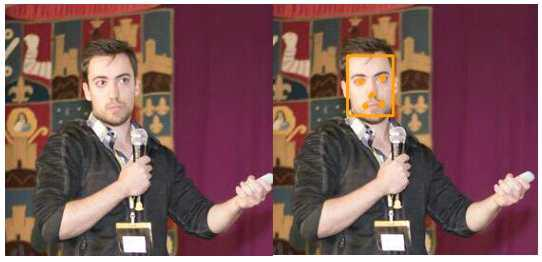
\includegraphics{pic/chp5/img881}
      \caption{MTCNN의 얼굴 감지 \protect\footnote{\protect\url {https://github.com/ipazc/mtcnn}}}
    \end{figure}

    \begin{figure}[h!]
      \centering
        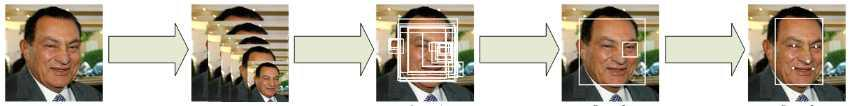
\includegraphics[scale = 0.7]{pic/chp5/img882}
      \caption{MTCNN 논문참고}
    \end{figure}



    MTCNN은 이미지에서 얼굴 부분만을 crop하는 방법 중 하나로 원 이미지를 여러 스케일로 변환하고 각 스케일에서 신경망을 적용하여 스케일마다 적절한 얼굴 특징점을 포착하여 전체 얼굴 부분을 찾아내는 방법이다. 신경망의 종류는 P-Net, R-Net, Q-Net이 있으며 이미지의 스케일에 따라 다른 신경망을 적용하여 특징점을 찾아내게 된다.

    \begin{figure}[h!]
      \centering
        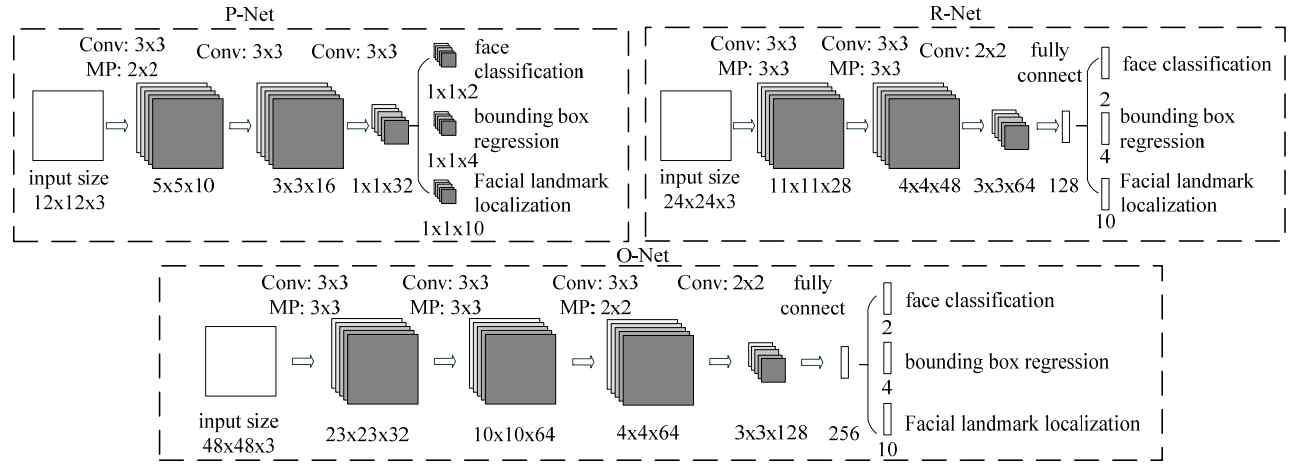
\includegraphics{pic/chp5/img885}
      \caption{MTCNN의 P-Net, R-Net, Q-Net}
    \end{figure}


    GAN을 이용한 얼굴 변형 모델에서는 학습에 데이터를 수집하기 위해 MTCNN을 사용하여 얼굴이미지를 수집한다. 먼저 얼굴을 바꾸고 싶은 소스 영상을 60FPS로 추출하여 초당 60개의 이미지를 소스영상을 통해 수집한다.

    \begin{figure}[h!]%사진X
    \centering
    %%\includegraphics{pic/chp7/}
    \caption{영상 자른거 결과사진}
    \end{figure}


    영상에서 얻은 모든 이미지를 활용하여 MTCNN을 통해 얼굴부분만을 crop한 새로운 이미지를 얻는다. 여기서 얼굴부분만 crop한 이미지는 원이미지에서 얼굴이 없을 경우 이미지가 만들어지지 않으다. 얼굴이 있는 이미지라도 MTCNN의 감지 에러로 인하여 얼굴 부분의 crop이 안되거나 얼굴이 아닌 다른 부분을 crop할 수 있는 경우가 있고 얼굴이 없는 이미지라도 MTCNN이 오판을 하여 특정 부분을 얼굴로 인식하여 해당부분을 crop한 이미지가 생성될 수 도 있다. 위와 같이 얼굴 부분만을 crop하여 생성된 이미지 중 잘못된 결과는 사용자가 판단하여 삭제를 한후 해당 이미지들로 학습에 사용하게 된다.

    \begin{figure}[h!]%사진X
    \centering
    %%\includegraphics{pic/chp7/}
    \caption{MTCNN으로 얼굴부분 감지된거랑 안된거 사진}
    \end{figure}


    \item 학습 과정에 필요한 얼굴 이미지의 binary mask 생성

    학습을 위해 먼저 생성된 얼굴이미지에서 $binary mask$를 생성하기 위해 $python$의 $face-alignment$ 패키지와 $dlib$ 패키지를 이용하게 된다.

    Binary mask 생성에 앞서 먼저 얼굴 이미지들을 사람의 정면 이미지처럼 변환하게 된다. dlib 패키지를 통해 얼굴이미지에서 사람의 얼굴 특징점을 파악하고 이 얼굴 특징점들이 사람이 정면을 보고 있는 이미지와 특징점들의 위치가 비슷해지도록 이미지 회전 및 이미지 확대, 축소를 통해 정면 얼굴이미지를 수집한다.
    \begin{figure}[h!] %사진X
    \centering
    %%\includegraphics{pic/chp7/}
    \caption{생성된 정면얼굴이미지}
    \end{figure}



    정면 얼굴 이미지가 모두 생성이 되면 dlib 패키지를 이용하여 해당 이미지들을 통해 binary mask 이미지를 생성하고 정면 얼굴이미지와 binary mask 이미지가 GAN 모델의 학습에 이용된다. 학습에 사용되는 이미지의 크기는 64*64 pixels이다. 
    \begin{figure}[h!]%사진X
    \centering
    %%\includegraphics{pic/chp7/}
    \caption{binary mask 생성결과}
    \end{figure}


    \item GAN 얼굴변형 모델의 Network Architecture

    GAN 얼굴변형 모델의 생성자와 구분자 신경망 구조는 다음과 같으며 생성자 신경망은 input 이미지의 통계적 분포를 판단하여 가짜이미지를 생성해 내며 구분자 신경망은 생성자가 만들어 낸 이미지가 가짜인지 실제 이미지인지 판단해 나가면서 두 신경망이 적대적으로 학습된다.
%%%%%%%%%%%%%%%%%%%%%%%%%%%%%%%%%%%%%%%%%%%%%%%%v
    \begin{figure}[h!]
    \centering
    \includegraphics{pic/chp5/img896}
    \includegraphics{pic/chp5/img897}
    \caption{생성자 신경망 구조 \cite{reference11}}
    \end{figure}
%%%%%%%%%%%%%%%%%%%%%%%%%%%%%%%%%%%%%%%%%%%%

    \begin{figure}[h!]
    \centering
    \includegraphics{pic/chp5/img906}
    \caption{구분자 신경망 구조\cite{reference11}}
    \end{figure}

    GAN 모델의 학습은 80000 iteration 진행하였다. 학습완료 후 생성된 신경망 모델을 이용하여 소스 동영상을 60FPS로 추출한 이미지들에서 얼굴 변형을 진행하고 완료시 얼굴이 변형된 결과 이미지들이 생성된다.

    위 과정이 완료되면 얼굴이 변형된 영상을 추출하기 위해 결과 이미지들을 python의 opencv 패키지를 재합성한다. 결과 이미지를 재합성 소스 영상에서 얼굴 부분만 변형된 새로운 영상을 추출할 수 있다.
\end{enumerate}

    \section{ GAN을 활용한 얼굴 변형 모델의 테스트 환경 및 결과}

    \subsection{테스트 환경}
    \spec
    \subsection{결과}
%%%%%%%%%%%%%%%%%%%%%%%%%%%%%%%%%%%%%%%%%%%%
    \begin{figure}[h!]
    \centering
        \includegraphics{pic/chp5/img907}
        \includegraphics{pic/chp5/img908}
    \caption{원 이미지(위), 얼굴 변형 된 이미지(아래)}
    \end{figure}
%%%%%%%%%%%%%%%%%%%%%%%%%%%%%%%%%%%%%%%%%%%%

    이 모델의 탐색을 통해, 얼굴이 좌우 90도 가까이 돌아가더라도 얼굴이 자연스럽게 변형되는 결과를 확인하였고, 일부 데이터에 장애물이 존재하더라도 어느 정도 보완하여 합성시켜준다는 점 또한 확인하였다. 하지만 이러한 결과를 얻기 위해선 충분한 데이터 셋의 수, 학습시간, 하드웨어의 성능이 필요할 것이다. 또한 얼굴 변형을 하는 소스 영상의 화질이 좋을수록 좋은 결과를 얻을 수 있었다. 하드웨어의 성능이 보장된다면 신경망 층의 크기를 늘린다면 더 세밀한 학습이 진행될 수 있을 것이며 학습 횟수 또한 모델의 성능에 있어서 중요한 요소가 될 수 있다.

\chapter{ 위 네 가지 기술들과 서버의 연결 및 결과  }

\section{ 서버설명 + cox 페이지 설명}


\begin{figure}[h!]
    \centering
    \includegraphics{pic/chp6/img921}
\end{figure}
\newpage
\begin{figure}[h!]
    \centering
    \includegraphics{pic/chp6/img928}
\end{figure}
「기능 1」

-MAIN PAGE로 REDIRECTION을 하는 기능을 가진다. LOGO로써의 기능을 겸한다.

「기능 2」

-MAIN PAGE의 TOP-BAR이며 CLICK시 해당되는 PAGE로 화면이 이동된다. 가독성 향상을 위한 기능이다.

「기능 3」

-COX PROJECT의 이름이 기안되어 있고 MAIN PAGE로 REDIRECTION을 하는 기능을 가진다.

「기능 4,5,6,7」

-각 기능 FACESWAP, GAN, OPENPOSE, ZAD PAGE로 연결되는 LINK BUTTON이다.

「그림 1」

-MAIN PAGE의 HOME PICTURE

「그림 2」

-COX에 대한 간략한 설명과 기능들에 대한 설명문

「그림 3」

-SERVICE들을 나타내며 각 기능의 명과 간략한 설명이 있고, 「기능 4,5,6,7」이 포함되어 있다.

「그림 4」

-이 그림 이후로 CONTACT 화면이 나올 것을 알려주는 그림

「그림 5」

-현재 연구하고 있는 연구실 위치를 나타내는 GOOGLE MAP과 주소, 담당자의 휴대전화와 이메일이 기재

「그림 6」

-WEB APPLICATION에 대한 저작권 NOTICE

\newpage

\begin{figure}[h!]
    \centering
    \includegraphics{pic/chp6/img934}
\end{figure}
「기능 1」

-얼굴을 합성할 사진 또는 영상을 선택해서 업로드하는 기능

「그림 1」

-기능과 그림이 위와 동일하다.

「그림 2」

-ZAD에 대한 설명과 간단한 기능 설명

「그림 3」

-위와 동일하다.

\newpage
\begin{figure}[h!]
    \centering
    \includegraphics{pic/chp6/img939}
\end{figure}

「기능 1」

-업로드된 사진 또는 영상을 미리본다.

「그림 1」

-기능과 그림이 위와 동일하다.

「그림 2」

-위와 동일하다.

\newpage
\begin{figure}[h!]
    \centering
    \includegraphics{pic/chp6/img945}
\end{figure}

「기능 1」

-얼굴이 합성된 영상 결과를 보여준다.

「그림 1」

-기능과 그림이 위와 동일하다.

「그림 2」

-위와 동일하다.

\section{ 2D-Faceswap 모델 실행 환경과 과정 및 결과}

\textbf{요구사항 :  opencv 및 dlib 설치 필요}

\subsection{인터프리터 (conda)환경}

\begin{table}[h!]
\centering
\begin{tabular}{|c|c|}
    \hline\hline
    dlib & 19.16.0 \\ \hline
    numpy & 1.15.4 \\             \hline
    opencv-python & 3.4.4.19\\             \hline
    pygame & 1.9.4 \\            \hline
    PyOpenGL & 3.1.0 \\            \hline
    scipy  &  1.1.0\\
    \hline\hline
\end{tabular}
\caption{2D-Faceswap의 인터프리터 세팅  }
\end{table}

\subsection{실행과정} 

앞서 Faceswap을 위해서 사용한 4가지 알고리즘 중 정면사진에 대한 변환인 2D-Faceswap 알고리즘을 적용하여 웹상에서 실시간으로 사용자에게 얼굴을 합성한 결과를 보여주도록 한다. 본 2D-Faceswap 알고리즘은 정면 영상에 대한 얼굴 합성에 이용되어진다. 

웹에 접속하여 2D-Faceswap 알고리즘을 적용하는 과정은 다음과 같다. 
\begin{enumerate}
    \item  사용자는 먼저 정면 동영상 A 와 합성하고 싶은 사진 B를 준비한다.
    \item 웹 상에 얼굴 정면이 들어가 있는 동영상 A와 사진 B를 업로드한다.
    \item 서버에서 2D-Faceswap 알고리즘을 동영상에 적용시킨다. (2D-Faceswap 알고리즘의 적용과정은 제2장에 있다.)
    \item 2D-Faceswap 알고리즘이 적용된 동영상을 웹 상에 표시한다.
\end{enumerate}

이때 2D-Faceswap 알고리즘은 영상에 여러 명의 사람이 등장할 경우 전체 사람의 얼굴을 변화시킨다는 단점이 있다. 따라서 우리는 2D-Faceswap 모델과 Openpose를 이용하여 여러 사람 중 한사람의 얼굴만을 합성시켜야 한다.



\section{ Openpose 를 활용한 Faceswap 모델 실행 환경과 과정 및 결과}

\textbf{요구사항 :  dlib 및 opencv 필요}

\subsection{인터프리터 (conda)환경}

\begin{table}[h!]
\centering
\begin{tabular}{|c|c|}
    \hline\hline
    face-recognition & 1.2.3\\ \hline
    face-recognition-models & 0.3.0 \\ \hline
    ffmpeg & 1.4 \\ \hline
    ffmpy & 0.2.2 \\ \hline
    dlib & 19.16.0 \\ \hline
    numpy & 1.15.4 \\ \hline
    opencv-python & 3.4.4.19\\ \hline
    pygame & 1.9.4 \\ \hline
    PyOpenGL & 3.1.0 \\ \hline
    scipy &1.1.0\\ \hline
    \hline\hline
\end{tabular}
\caption{Openpose의 인터프리터 셋팅 }
\end{table}

앞서 2절에서 사용한 $2D-Faceswap$의 경우 영상에서 얼굴이 여러명이 나올 경우 여러명의 얼굴이 동시에 변환된다는 단점이 있다. 따라서 우리는 Tensorflow 의 $face_recognition$ 와 Openpose를 통해서 사람들의 얼굴을 인식한 후 사용자가 추가한 사진과 유사한 얼굴을 감지하여 해당하는 얼굴만을 변환하도록 한다.

웹에 접속하여 Openpose를 활용한 Faceswap 모델 적용하는 방법은 다음과 같다.

\begin{enumerate}
    \item 사용자는 먼저 바꾸고 싶은 얼굴과 합성하고 싶은 얼굴을 업로드한다.
    \item 합성하고자하는 동영상을 선택한다.
    \item 합성하고자 하는 동영상에서 사용자가 올린 사진과 비교하여 바꾸고 싶은 얼굴을 감지한다.
    \item 얼굴을 감지 한 후 2절에서 사용한 2D-Faceswap을 이용하여 얼굴을 합성한다.
    \item 합성한 결과를 웹 상에 표시한다.
\end{enumerate}

\section{딥페이크(Original-High-Resolution Model) 모델 실행 환경과 과정 및 결과}

\textbf{요구사항 : Nvidia GPU 사용 시 CUDA 세팅}


\subsection{인터프리터 (conda)환경 -Nvidia GPU사용 CUDA 세팅}

\begin{table}[h!]
\centering
\begin{tabular}{|c|c|}
    \hline\hline
    Click & 7.0 \\ \hline
    cloudpickle & 0.6.1 \\ \hline
    cmake & 3.13.1 \\ \hline
    cycler& 0.10.0 \\ \hline
    dask & 1.0.0 \\ \hline
    decorator & 4.3.0 \\ \hline
    dlib & 19.16.0 \\ \hline
    face-recognition &  1.2.3 \\ \hline
    face-recognition-models & 0.3.0 \\ \hline
    ffmpy & 0.2.2 \\ \hline
    h5py & 2.8.0 \\ \hline
    Keras & 2.2.4 \\ \hline
    Keras-Applications & 1. 0.6 \\ \hline
    Keras-Preprocessing & 1.0.5 \\ \hline
    kiwisolver & 1.0.1 \\ \hline
    matplotlib & 2.2.2 \\ \hline
    networkx &  2.2 \\ \hline
    numpy & 1.15.4 \\ \hline
    nvidia-ml-py3 & 7.352.0 \\ \hline
    opencv-python & 3.4.4.19 \\ \hline
    pathlib & 1.0.1 \\ \hline
    Pillow & 5.3.0 \\ \hline
    psutil & 5.4.8 \\ \hline
    pyparsing & 2.3.0 \\ \hline
    python-dateutil & 2.7.5 \\ \hline
    pytz & 2018.7 \\ \hline
    PyWavelets &  1.0.1 \\ \hline
    PyYAML &  3.13 \\ \hline
    scandir & 1.7 \\ \hline
    scikit-image & 0.14.1 \\ \hline
    scikit-learn & 0.20.1 \\ \hline
    scipy & 1.1.0 \\ \hline
    six & 1.12.0 \\ \hline
    toolz  & 0.9.0 \\ \hline
    tqdm & 4.28.1 \\ \hline
    \hline\hline
\end{tabular}
\caption{딥페이크의 인터프리터 셋팅 }
\end{table}

\subsection{실행과정}

Faceswap을 위해서 사용한 4가지 알고리즘 중 deepfake 알고리즘을 사용하여 얼굴을 바꿀 데이터를 직접 학습시켜 사용자에게 얼굴을 합성한 결과물을 자연스럽고 높은 퀄리티로 사용자들에게 보여준다.

\begin{enumerate}
    \item  사용자는 먼저 정면 동영상 A와 얼굴 A를 B로 바꿔주는 트레이닝 된 모델을 준비한다.
    \item 웹 상에 얼굴 정면이 들어가 있는 동영상 A와 모델을 업로드한후 결과가 저장될 폴더를 정한다..
    \item 서버에서 deepfake 알고리즘을 동영상에 적용시킨다.  (deepfake 알고리즘의 적용과정은 제4장에 있다.)
    \item deepfake 알고리즘이 적용된 동영상을 웹 상에 표시하고 결과물을 폴더에 저장시킨다..
\end{enumerate}

세부 작동방식 :

\begin{enumerate}
    \item  동영상 A를 사진으로 잘게 자른다. 
    \item  모델을 사용해서 각 사진의 A의 얼굴을 B로 바꾼다. 
    \item  사진을 다시 동영상으로 합친 후 웹에서 실행하고 폴더에 저장한다
\end{enumerate}

\section{생성적 적대 신경망(GAN) 모델 실행 환경과 과정 및 결과}

\subsection{요구사항 : 아나콘다 가상환경 구축}


윈도우 환경에서 python 모듈인 pytorch 모듈이 설치가 안 되므로 Anconda를 이용하여 가상환경을 구축하였고, 아나콘다로 파이썬 3.6버전의 가상환경을 생성하였다.

\subsection{인터프리터 (conda)환경}

\begin{table}[h!]
\centering
\begin{tabular}{|c|c|}
    \hline\hline
    dlib & 19.15.0 \\ \hline
    face-alignment & 1.0.0  \\ \hline
    face-recognition & 1.2.3  \\ \hline
    face-recognition-models & 0.3.0  \\ \hline
    Keras & 2.1.5  \\ \hline
    Keras-Applications & 1.0.6  \\ \hline
    Keras-Preprocessing & 1.0.5  \\ \hline
    keras-vggface  & 0.5  \\ \hline
    matplotlib & 2.2.2  \\ \hline
    moviepy & 0.2.3.5  \\ \hline
    nvidia-ml-py &  375.53.1  \\ \hline
    nvidia-ml-py3 &  7.352.0  \\ \hline
    opencv-python & 3.4.1.15  \\ \hline
    pathlib & 1.0.1 \\ \hline 
    prefetch-generator &  1.0.1  \\ \hline
    pygame & 1.9.4  \\ \hline
    tensorflow-gpu &  1.12.0  \\ \hline
    torch & 0.4.1  \\ \hline
    \hline\hline
\end{tabular}
\caption{GAN의 인터프리터 셋팅 }
\end{table}


\subsection{실행 과정}
\begin{enumerate}%[label={\pgana*.}]

    \item 실행코드 변경

    앞서 5절에서 사용한 GAN을 이용한 얼굴 변형 모델\cite{reference13}은 웹에서 실행 할 수 없는 주피터 노트북으로 작성된 파이썬 코드이다. 따라서 핵심 모듈을 일괄작업 방식으로 코드 실행 시 파일의 경로를 받아 작업을 수행하도록 코드를 새로 작성하였다.

    \item 핵심 모듈 구성

    앞서 5절에서 설명한 3가지 과정과 비디오를 변환하는 모듈을 작성하였다.
    -MTCNN face detection


    -prep binary masks

    -Train module

    -Video conversion

    \item 모듈 동작 과정
    \begin{enumerate}
        \item  사용자는 얼굴을 바꾸고 싶은 동영상을 업로드한다. 이하 A동영상
        \item 합성하고자 하는 인물의 동영상을 업로드한다. 이하 B동영상
        \item MTCNN face detection 모듈을 실행하여 A동영상과 B동영상에서 얼굴을 추출한다.
        \item prep binary masks 모듈을 실행하여 얼굴을 정렬한다.
        \item Train module을 실행하여 학습된 모델을 생성한다.
        \item Video conversion 모듈을 실행하면 학습된 모델을 이용하여 A동영상에 B를 합성한다.
        \item 합성한 결과를 웹 상에 표시한다.
    \end{enumerate}

\end{enumerate}
3. 실행 결과

사진

\chapter{ COX Cinema 및 interactive 광고 동영상 제작 및 업로드}

\section{ COX Cinema 설명 + Branch 기능}

\subsection{정의}

COX cinema란 광고와 사용자 간의 상호작용이 가능하게 하는 인터렉티브 미디어 플랫폼입니다. 	


\subsection{ 세부내용}

COX Cinema에서 쓰이는 기능 중 하나인 Branch Service는 제작자가 일반적으로 생각하는 영상과는 다른 영상을 만들 수 있게 해준다. 일반적인 영상이 영상제작자가 사용자에게 영상의 결과를 제공하는 다소 단방향적인 것이었다면, COX Cinema의 Branch Service는 영상제작자가 여러 Branch를 만들어서 영상을 만들게 한다. 일반적인 영상을 보는 사용자는 영상을 보고 느끼는 것이 다라면, 사용자가 COX Cinema를 이용하면 직접 영상의 진행에 참여하고 사용자가 결과를 만드는 것에 참여하는 느낌을 받게 한다.     

\begin{figure}[h!]
    \centering
        \includegraphics{pic/chp7/img994}
    \caption{COX Cinema – Branch 기능}
\end{figure}

\begin{figure}[h!]
\centering
\includegraphics{pic/chp7/img1004}
\caption{Android 화면 – Branch }
\end{figure}

\begin{figure}[h!]
\centering
\includegraphics{pic/chp7/img1003}
\caption{Web 화면 – Branch 기능}
\end{figure}


\section{ COX Cinema 기능 구현}
영상제작자가 플랫폼 상에서 편집이 이루어질 때에 시점과 범위의 두 가지 관점에서 Interactive기능이 구현된다. Interactive 기능은 영상제작자가 사용자에게 어떤 영상에서 영상제작자와 사용자간의 대화라고 볼 수 있다. push, call, image 등 여러 가지 Interactive기능을 만들었으며 자세한 사항은 아래에 설명한다.  

\subsection{시점 지정}

영상제작자가 원하는 시점(시간)에서 Interactive기능을 부여한다. Interactive 기능은 영상제작자가 사용자에게 어떤 영상에서 영상제작자와 사용자간의 대화라고 볼 수 있다. push, call, image 등 여러 가지 Interactive기능을 만들었으며 자세한 사항은 아래에 설명한다.  

\begin{enumerate}

    \item  Push 

    영상제작자가 사용자에게 메시지를 보내 제작자가 원하는 메시지를 사용자에게 보내는 기능

    PUSH 동작 pic

    \begin{figure}[h!]
    \centering
    \includegraphics{pic/chp7/img1001}
    \caption{android 화면 - push}
    \end{figure}
    \begin{figure}[h!]
    \centering
    \includegraphics{pic/chp7/img1002}
    \caption{web 화면 - push}
    \end{figure}

    \item  Push Link 

    영상제작자가 사용자에게 링크를 보내 사용자에게 링크접속을 유도하는 기능

    \begin{figure}[h!]
    \centering
    \includegraphics{pic/chp7/img1013}
    \caption{android 화면 – pushlink}
    \end{figure}

    \begin{figure}[h!]
    \centering
    \includegraphics{pic/chp7/img1014}
    \caption{android 화면 – pushlink 2}
    \end{figure}

    \begin{figure}[h!]
    \centering
    \includegraphics{pic/chp7/img1015}
    \caption{web 화면 – pushlink}
    \end{figure}

    \item  Morse

    영상제작자가 morse 부호를 설정하여 사용자의 기기에서 소리가 나게 하는 기능
    Morse 동작 pic

    \item  Call 

    사용자기기로 영상제작자가 원하는 이름과 전화번호를 설정하여 전화모드가 구현되는 기능

    \begin{figure}[h!]
    \centering
    \includegraphics{pic/chp7/img1018}
    \caption{Web 화면 – Call}
    \end{figure}


    \begin{figure}[h!]
    \centering
    \includegraphics{pic/chp7/img1017}
    \caption{android 화면 – Call}
    \end{figure}


    \item  Image 

    사용자기기로 영상제작자가 원하는 이미지를 보내주는 기능

    \begin{figure}[h!]
    \centering
    \includegraphics{pic/chp7/img1028}
    \caption{android 화면 – Image}
    \end{figure}

    \begin{figure}[h!]
    \centering
    \includegraphics{pic/chp7/img1029}
    \caption{web 화면 – Image}
    \end{figure}



    \item Motion 

    영상제작자가 사용자에게 모바일 기기를 움직이게 하여 영상에 참여하도록 유도하는 기능
    \begin{figure}[h!]
    \centering
    \includegraphics{pic/chp7/img1030}
    \caption{android 화면 – Motion}
    \end{figure}
    \begin{figure}[h!]
    \centering
    \includegraphics{pic/chp7/img1031}
    \caption{web 화면 – Motion}
    \end{figure} 

    \item Product

    사용자가 영상시청중 제품을 구매하게 유도하는 기능 

    \begin{figure}[h!]
    \centering
    \includegraphics{pic/chp78/img1123}
    \caption{web 화면 – product}
    \end{figure} 

\end{enumerate}

\subsection{범위 지정}

\begin{enumerate}
    \item Drawing X 안됨

    기능설명
    동작 pic


    \item Linkbox
    기능설명 모바일기기에서 안됨

    \item Vote

    사용자로 하여금 선택권을 주어 투표에 의해 영상이 선택되게 하는 기능.

    동작 pic

    \begin{figure}[h!]
    \centering
    %\includegraphics{pic/chp7/}
    \caption{web 화면 – Vote}
    \end{figure} 


    \begin{figure}[h!]
    \centering
    %\includegraphics{pic/chp7/}
    \caption{web 화면 – Vote}
    \end{figure} 

\end{enumerate}

\newpage

\section{ COX Cinema로 만든 영상 예시의 실행환경 및 결과 }

\subsection{테스트 환경 }
\spec
모바일 기기의 경우 Android 기기를 이용하여야한다.

\subsection{ 구성 및 제작 결과}

\begin{enumerate}

\item 구성도

\begin{figure}[h!]
\centering
%\includegraphics{pic/chp7/}
\caption{web 화면 – Vote}
\end{figure} 

\item 스토리 구성

    \begin{enumerate}%[label={\pgana*.}]

        \item 주제 : 배고픈 식사시간에 어떤 음식을 먹을 것인지에 대한 주제로 이야기가 전개된다.  
        \item 등장인물 : 여자주인공, 남자주인공1, 남자주인공2, 그 외 다수
        \item 원 영상 출처 : tvN 드라마 ‘식샤를 합시다1,2’ 

        \item 줄거리 : 여자 주인공이 운동을 하다가 휴대폰을 보게 되고 “배고프다~밥먹으러가자!“ 라는 메시지를 받으면서 이야기가 시작된다. 메시지를 받은 사용자의 모바일기기에 3가지 메뉴 중 먹고 싶은 메뉴를 고를 수 있는 선택권이 주어지게 되고 주인공은 치킨, 탕수육, 휴게소 음식(알 감자) 중 원하는 음식을 고르게 된다. 첫 번째로 치킨을 고르게 될 경우 치킨을 먹게 된다. 여자 주인공과 남자주인공1이 치킨을 나눠먹는 사이, 다른 한명의 남자주인공이 뒤늦게 치킨 무를 받아오며 늦게 합류해 함께 치킨을 먹는 모습이 보여 진다. 

    두 번째로는 탕수육이다. 여자주인공과 남자주인공이 사람들과 탕수육을 먹으러 중국집에 가게 된다. 주문한 음식들이 나와져있고 그중 탕수육을 먹게 되는데, 남자주인공이 탕수육 고기에 소스를 부으려는 순간 여자주인공이 크게 반발하며 다투다가 사용자의 모바일기기에 소스를 부어먹을 것인지, 소스에 찍어먹을 것인지 결정하는 투표기능이 주어지게 된다. 이후 하나는 소스를 탕수육에 맛있게 부어먹는 줄거리가 진행이 되고 하나는 소스에 맛있게 찍어먹는 줄거리가 펼쳐진다. 

    마지막으로는 휴게소 음식이다. 여자주인공이 휴게소음식(알 감자)를 받아와서 먹으려는 중 전화가 오게 되고 전화통화가 끝난 여자 주인공은 다시 알 감자를 먹으려고 하는 찰나, 사용자의 모바일 기기에 흔들어달라는 기능이 나타나게 된다. 사용자가 흔드는 행동을 취하게 되면 여자 주인공이 실수로 알 감자를 팔로 쳐 떨어트리게 되고 속상해하던 여자 주인공은 아까워하며 몰래 알 감자를 주워 먹다가 지나가는 아이에 의해 놀림을 받고 끝나게 된다.

        \item 목적 : 요즈음 대중매체로의 정보전달이 활발하고 참여율이 높은 만큼 일명 ‘먹방’ (먹는 방송)이 확대되고 있다. 단순히 먹는 것이 생존 및 영양소 섭취의 의미가 아니라 삶에서 큰 비율을 차지하며 행복의 수단으로서의 역할이 대두되고 있다. 이처럼 내가 원하는 음식을 원하는 방법으로 먹는 것을 볼 수 있다는 편리함을 주고, 단순히 편리함에서 그치는 것이 아니라 드라마 형식의 먹는 방송을 구현해낼 수 있다는 큰 장점을 가진다. 그 과정에서 거부감 없이 광고효과가 이뤄지고 또 그러한 사용자의 심리에 부응해 주문까지도 간편하게 가능할 수 있게 해 주는 다기능을 사용한 최초의 멀티 인터렉티브 무비이다.  
    \end{enumerate}

\item 기능 구성

    \begin{enumerate}%[label={\pgana*.}]
        \item BRANCH 기능

        \begin{figure}[h!]
            \centering
        \includegraphics{pic/chp78/img1081}
            \caption{web 화면 – Branch}
        \end{figure} 

        \begin{figure}[h!]
            \centering
        \includegraphics{pic/chp78/img1082}
            \caption{web 화면 – Branch}
        \end{figure} 

        여자주인공이 배가 고프니, 밥을 먹으러 가자는 메시지를 받고나서 어떤 음식을 먹을지 선택을 하도록 하기 위하여 사용한 Branch 기능이다. 이제 COX 애플리케이션을 사용하는 모바일 기기 사용자는 이 기능으로 하여금 어떻게 이야기를 전개할 것인지 선택을 할 수 있게 된다. 

        \item PUSH (메세지 기능 )

        \begin{figure}[h!]
            \centering
        \includegraphics{pic/chp78/img1094}
            \caption{android 화면 – Push}
        \end{figure} 

    이 기능은 앞서 ‘가.’ 에서 언급되었던 메시지이다. 여자 주인공이 운동을 하다가 휴대폰에 온 이 메시지를 보고서 어떤 메뉴를 먹을 것인지 선택하게 된다. 모바일 애플리케이션 사용자는 기기로 이 메시지를 받게 된다.

        \item PUSH LINK 기능
        
        \begin{figure}[h!]
            \centering
        \includegraphics{pic/chp78/img1095}
            \caption{android 화면 – PUSH LINK}
        \end{figure} 

    치킨 메뉴에서 여자주인공과 남자주인공들이 치킨을 먹는 중에 모바일 기기 사용자로 하여금 극중 여자 주인공이 치킨을 먹으면서 입고 있는 옷의 정보를 이 기능으로 제공해줄 수 있다. 위의 사진에서 YES 버튼을 누르게 되면 옷의 정보가 담긴 인터넷 URL로 자동으로 접속이 되며 인터넷 창이 뜨게 된다.

        \item VOTE 기능

        \begin{figure}[h!]
            \centering
        \includegraphics{pic/chp78/img1106}
            \caption{web 화면 – Vote}
        \end{figure} 

        \begin{figure}[h!]
            \centering
        \includegraphics{pic/chp78/img1106}
            \caption{web 화면 – Vote}
        \end{figure} 

    탕수육을 먹는 에피소드에서 탕수육을 어떻게 먹을 것 인지 투표를 하는 기능으로 쓰였다. 약 10초정도의 시간이 주어지고 모바일기기 사용자는 시간 안에 투표를 하면 된다. 이 투표결과를 바탕으로 자연스럽게 BRANCH의 기능 역시 가질 수 있다. 갈래를 자동으로 구분해주어 별도로 BRANCH 선택을 하지 않아줘도 되어 편리하다. 

        \item MOTION 기능

        \begin{figure}[h!]
            \centering
        \includegraphics{pic/chp78/img1108}
            \caption{web 화면 – MOTION}
        \end{figure} 

        \begin{figure}[h!]
            \centering
        \includegraphics{pic/chp78/img1107}
            \caption{web 화면 – MOTION}
        \end{figure} 


    휴게소 음식 (알 감자) 줄거리 부분에서 여자주인공이 전화를 끝낸 직후 위와 같이 화면상에 “흔들어주세요!“

    라는 문구가 뜨게 된다. 모바일 사용자는 해당 문구를 본 후에, 자신의 모바일 기기를 흔들게 된다. 흔들면 감자가 쏟아지는 줄거리가 전개될 때 이와 같은 기능을 사용하였다.

        \item PRODUCT 기능
        
        \begin{figure}[h!]
            \centering
        \includegraphics{pic/chp78/img1123}
            \caption{web 화면 – Product}
        \end{figure} 

    마지막으로 이 기능은 치킨 메뉴의 줄거리가 전개될 때에 사용자가 치킨이 먹고 싶어지겠다는 생각이 들 때 즈음, 곧바로 주문을 할 수 있게 끔 해주는 기능이다. 어떤 영상을 보고 있을 때 내가 보는 영상에서 사고 싶은 혹은 먹고 싶은 것을 손쉽게 구매할 수 있게 하는 기능은 어떤 기능보다도 광고효과를 비롯해 구매 욕구를 불러일으킬 수 있다. 사용자(소비자) 입장에서도 손쉽게 구매를 할 수 있다는 점에서 효율적이고 편리한 기능이라고 할 수 있다.
    \end{enumerate}
\end{enumerate}

\begin{thebibliography}{}
    \bibitem{reference1}
    Sun, X., Wu, P., \& Hoi, S. C. (2018). Face detection using deep learning: An improved faster RCNN approach. Neurocomputing, 299, 42-50.
        
    \bibitem{reference2} 
    Gosavi, V. R., Sable, G. S., \& Deshmane, A. K. (2018). Evaluation of Feature Extraction Techniques using Neural Network as a Classifier: A Comparative Review for face Recognition.

    \bibitem{reference3} 
    Zhang, X., Sun, Y., \& He, W. (2018, August). Face Alignment Based on Two-Stage Localization. In Journal of Physics: Conference Series (Vol. 1069, No. 1, p. 012164). IOP Publishing.

    \bibitem{reference4} 
    Nirkin, Y., Masi, I., Tuan, A. T., Hassner, T., \& Medioni, G. (2018, May). On face segmentation, face swapping, and face perception. In Automatic Face \& Gesture Recognition (FG 2018), 2018 13th IEEE International Conference on (pp. 98-105). IEEE.

    \bibitem{reference5}
    Dong, H., Neekhara, P., Wu, C., \& Guo, Y. (2017). Unsupervised image-to-image translation with generative adversarial networks. arXiv preprint arXiv:1701.02676.

    \bibitem{reference6} 
    Wang, M., \& Deng, W. (2018). Deep Face Recognition: A Survey. arXiv preprint arXiv:1804.06655.

    \bibitem{reference7} 
    Kazemi, V., \& Sullivan, J. (2014). One millisecond face alignment with an ensemble of regression trees. In Proceedings of the IEEE Conference on Computer Vision and Pattern Recognition (pp. 1867-1874).

    \bibitem{reference8}
    Blanz, V., \& Vetter, T. (1999, July). A morphable model for the synthesis of 3D faces. In Proceedings of the 26th annual conference on Computer graphics and interactive techniques (pp. 187-194). ACM Press/Addison-Wesley Publishing Co..

    \bibitem{reference9} 
    \url{https://github.com/MarekKowalski/FaceSwap}

    \bibitem{reference10} 
    \url{https://github.com/ZheC/Realtime_Multi-Person_Pose_Estimation}

    \bibitem{reference11} 
    \url{https://github.com/deepfakes/faceswap}

    \bibitem{reference12} 
    \url{http://mangastorytelling.tistory.com/m/6984}

    \bibitem{reference13} 
    \url{https://github.com/shaoanlu/faceswap-GAN}

\end{thebibliography}
    
\end{document}
